\section{Размерное квантование в двумерных системах.  Энергетический спектр, плотность состояний, концентрация двумерных электронов. Примеры двумерных структур.}

\textbf{Размерное квантование в двумерных системах.}
Основная идея базируется на основе волновых свойств электрона.
Ограничение размера требует размещения целого числа полуволн в
пределах структуры.
\begin{figure} [h!]
    \centering
    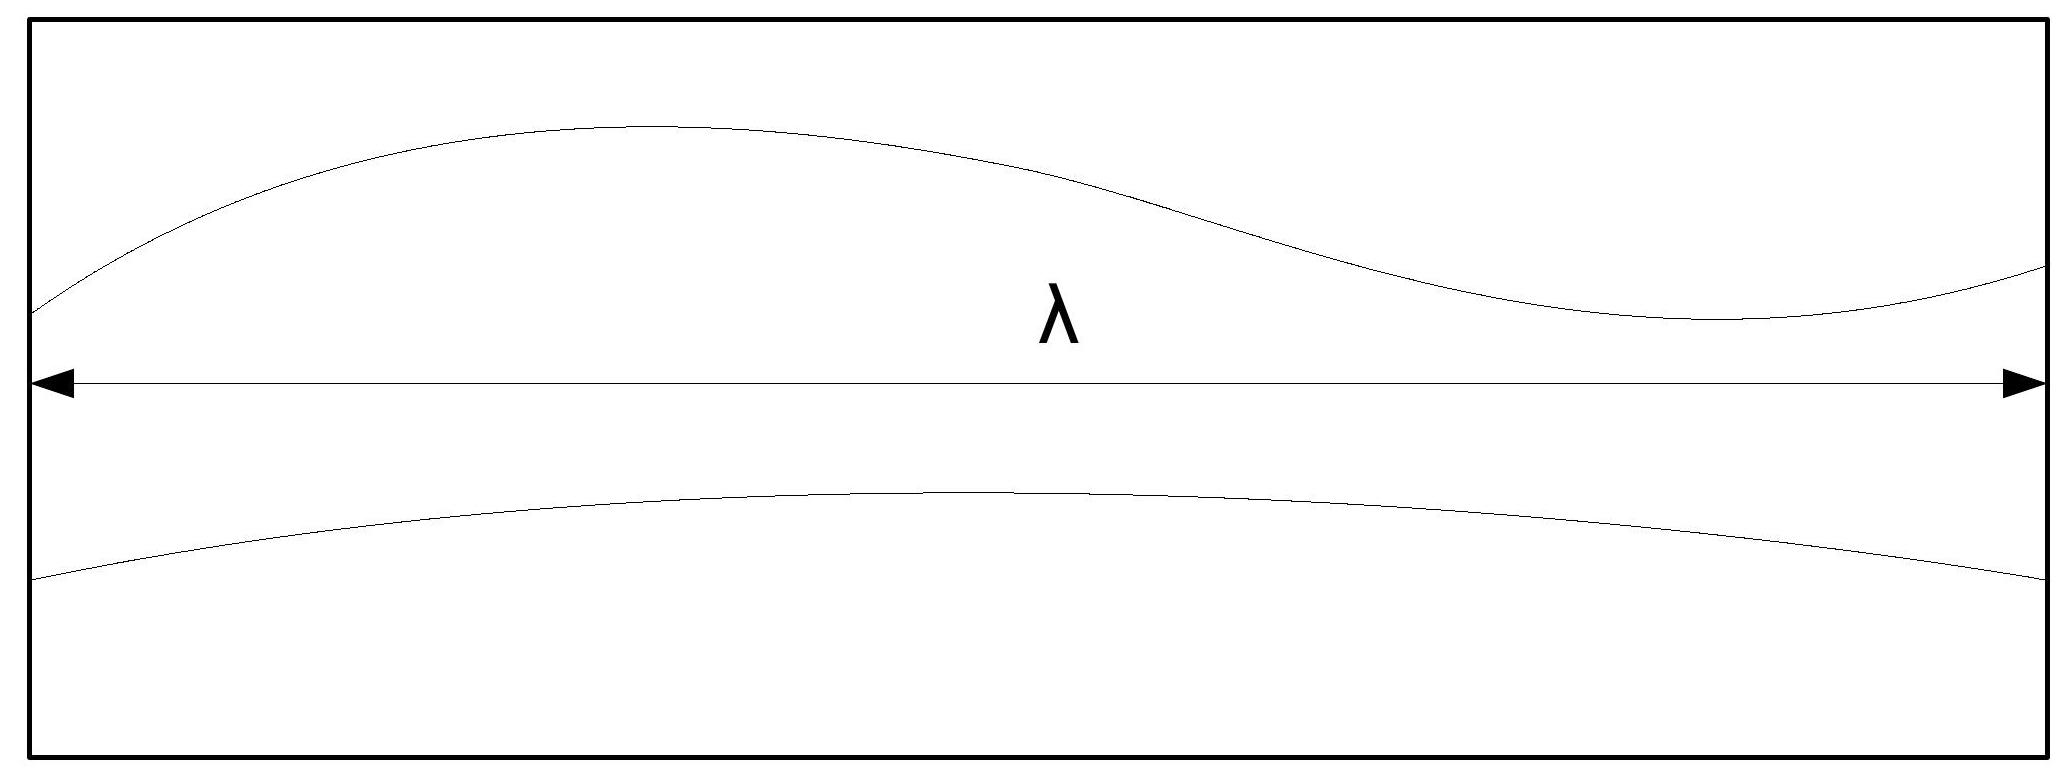
\includegraphics[width=0.7\textwidth]{2023_05_21_66a3dfca5be088b7d6b7g-01}
\end{figure}

В результате энергетический спектр становится дискретным

$$
U(x, y, z)=\left\{\begin{array}{cc}
0, & 0 \leq z \leq L_{z} \\
U_{0,} & z<0, z>L_{z}
\end{array}\right\}
$$

\begin{figure}[h!]
    \centering
    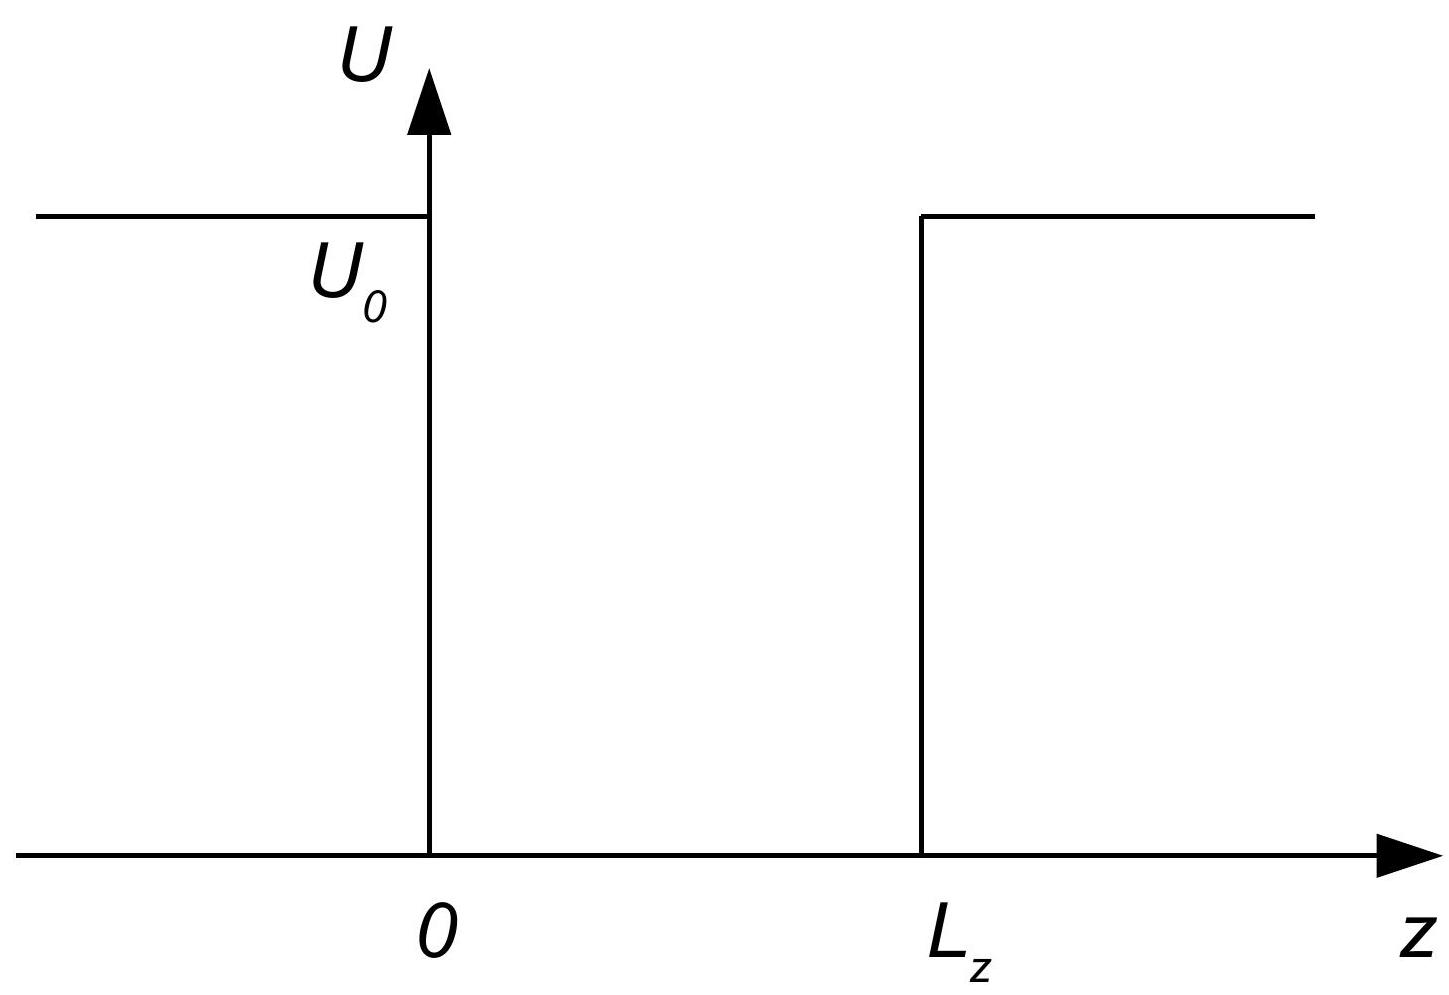
\includegraphics[width=0.5\textwidth]{2023_05_21_66a3dfca5be088b7d6b7g-02}
\end{figure}


Нет зависимости потенциальной энергии от х, у в явном виде, поэтому:

$$
\psi(x, y, z)=\exp \left(i\left(k_{x} x+k_{y} y\right)\right) \psi_{z}(z)
$$

$k_{x}, k_{y}$ - компоненты волнового вектора вдоль $\mathrm{x}, \mathrm{y}$

Оператор Гамильтона и уравнение Шредигера
$$
\begin{aligned}
\hat{H}= & -\frac{\hbar^{2}}{2 m_{e}}\left(\frac{\partial^{2}}{\partial x^{2}}+\frac{\partial^{2}}{\partial y^{2}}+\frac{\partial^{2}}{\partial z^{2}}\right)+U(x, y, z) \\
& \hat{H} \psi(x, y, z)=E \psi(x, y, z)
\end{aligned}
$$

Подстановка волновой функции в уравнение даёт

$$
\frac{d^{2} \psi_{z}}{d z^{2}}+\frac{2 m_{e}}{\hbar^{2}}\left(E-\frac{\hbar^{2}}{2 m}\left(k_{x}^{2}+k_{y}^{2}\right)-U(z)\right) \psi_{z}=0
$$
\textbf{Потенциальный ящик с бесконечными стенками $
U_{0} \rightarrow \infty$}

Волновая функция должна быть равна нулю в области с бесконечной потенциальной энергией:

$$
\psi_{z}=\left\{\begin{array}{c}
c_{m s} \sin \left(k_{z} z\right)+c_{m c} \cos \left(k_{z} z\right), \quad 0 \leq z \leq L_{z} \\
0, \quad z<0, z>L_{z}
\end{array}\right.
$$

Граничное условие при z=0 даёт $c_{m c}=0$. 

Граничное условие при $z=L_{z}$ даёт:
$
k_{z}=\frac{\pi n}{L_{z}}, n=1,2,3 \ldots
$

Условие нормировки даёт: $\quad c_{m s}=\sqrt{\frac{2}{L_{z}}}$
Тогда решение:
$$
\begin{gathered}
\psi_{z}=\left\{\begin{array}{c}
\sqrt{\frac{2}{L_{z}}} \sin \left(\frac{\pi n z}{L_{z}}\right), \quad 0 \leq z \leq L_{z} \\
0, z<0, z>L_{z}
\end{array}\right. \\
E-\frac{\hbar^{2}}{2 m_{e}}\left(k_{x}^{2}+k_{y}^{2}\right)=\frac{\hbar^{2} k_{z}^{2}}{2 m_{e}} \quad \\
\text{Энергетический спектр: }E=\frac{\hbar^{2}}{2 m_{e}}\left(k_{x}^{2}+k_{y}^{2}\right)+\frac{\pi^{2} \hbar^{2} n^{2}}{2 m_{e} L_{z}^{2}}, n=1,2,3 \ldots
\end{gathered}
$$
\begin{figure} [h!]
    \centering
    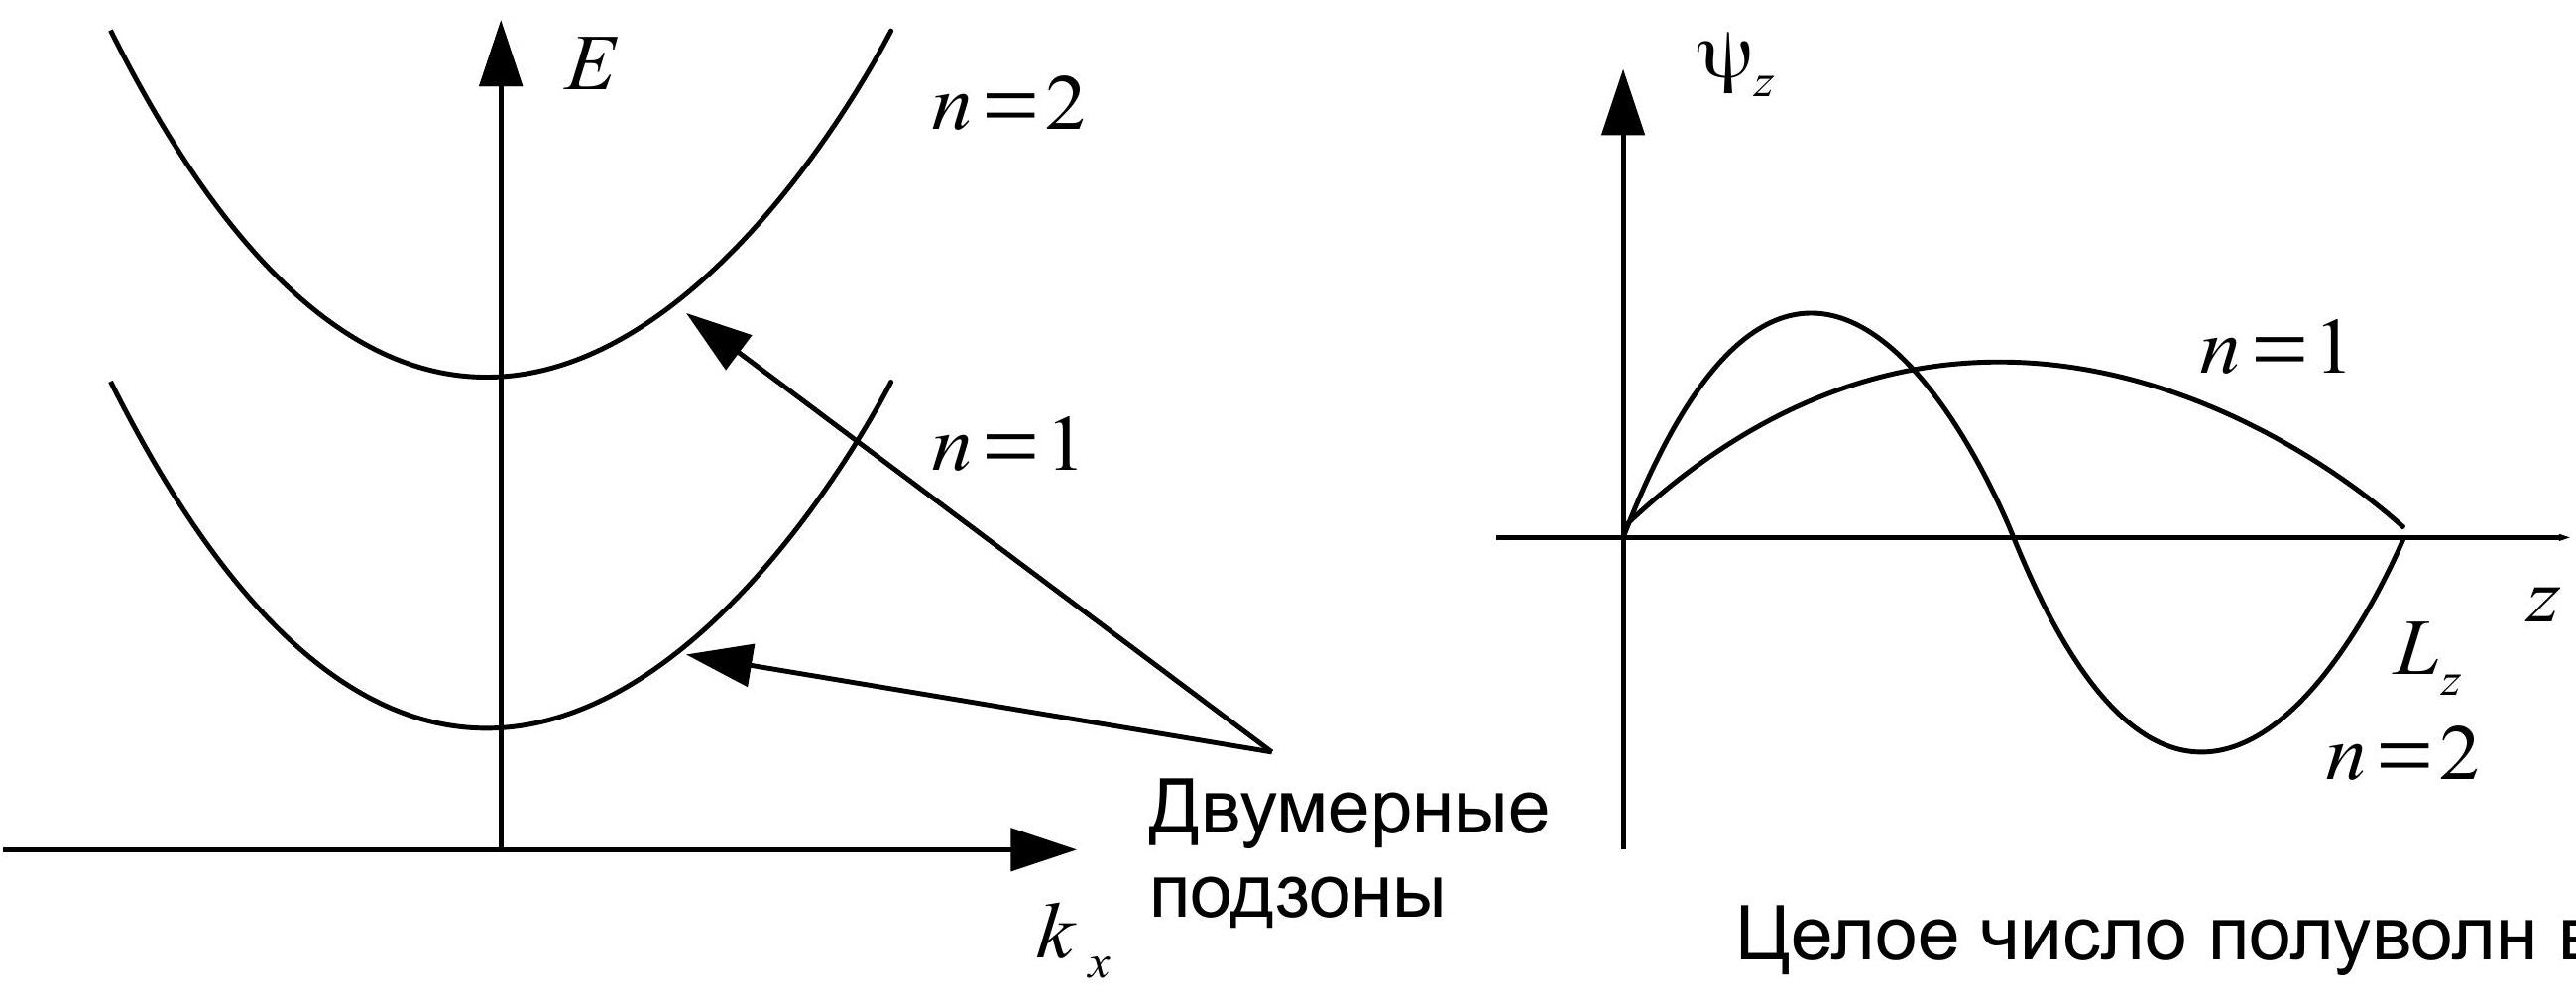
\includegraphics[width=0.7\textwidth]{2023_05_21_66a3dfca5be088b7d6b7g-05}
\end{figure}


\textbf{Решения внутри ящика $E<U_{0}$}
$$
\psi_{z}=\left\{\begin{array}{c}
c_{l} \exp \left(\frac{\sqrt{2 m\left(U_{0}-E\right)}}{\hbar} z\right), \quad z<0 \\
c_{m s} \sin \left(\frac{\sqrt{2 m E}}{\hbar} z\right)+c_{m c} \cos \left(\frac{\sqrt{2 m E}}{\hbar} z\right), 0 \leq z \leq L_{z} \\
c_{r} \exp \left(-\frac{\sqrt{2 m\left(U_{0}-E\right)}}{\hbar} z\right), \quad z>L_{z}
\end{array}\right\}
$$

Непрерывность волновой функции и её производной при z=0 и z= $L_{z}$ даёт систему линейных однородных уравнений относительно коэфициентов $c$ :

$$
\begin{aligned}
&c_{l}=c_{m c} \\
&c_{l} \sqrt{2 m \frac{\left(U_{0}-E\right)}{\hbar}}=c_{m s} \frac{\sqrt{2 m E}}{\hbar} \\
&c_{m s} \sin \left(\frac{\sqrt{2 m E}}{\hbar} L_{z}\right)+c_{m c} \cos \left(\frac{\sqrt{2 m E}}{\hbar} L_{z}\right)=c_{r} \exp \left(-\frac{\sqrt{2 m\left(U_{0}-E\right)}}{\hbar} L_{z}\right) \\
&c_{m s} \frac{\sqrt{2 m E}}{\hbar} \cos \left(\frac{\sqrt{2 m E}}{\hbar} L_{z}\right)-c_{m c} \frac{\sqrt{2 m E}}{\hbar} \sin \left(\frac{\sqrt{2 m E}}{\hbar} L_{z}\right)=\\
&-c_{r} \frac{\sqrt{2 m\left(U_{0}-E\right)}}{\hbar} \exp \left(-\frac{\sqrt{2 m\left(U_{0}-E\right)}}{\hbar} L_{z}\right)
\end{aligned}
$$

Ненулевые решения при определителе матрицы системы уравнений равном нулю. Это даёт уравнение на $E$, которое имеет несколько решений.При любом $E>U_{0}$ существует ненулевое решение незатухающее при
 удалении от потенциального ящика (трёхмерного)

 \begin{figure} [h!]
    \centering
    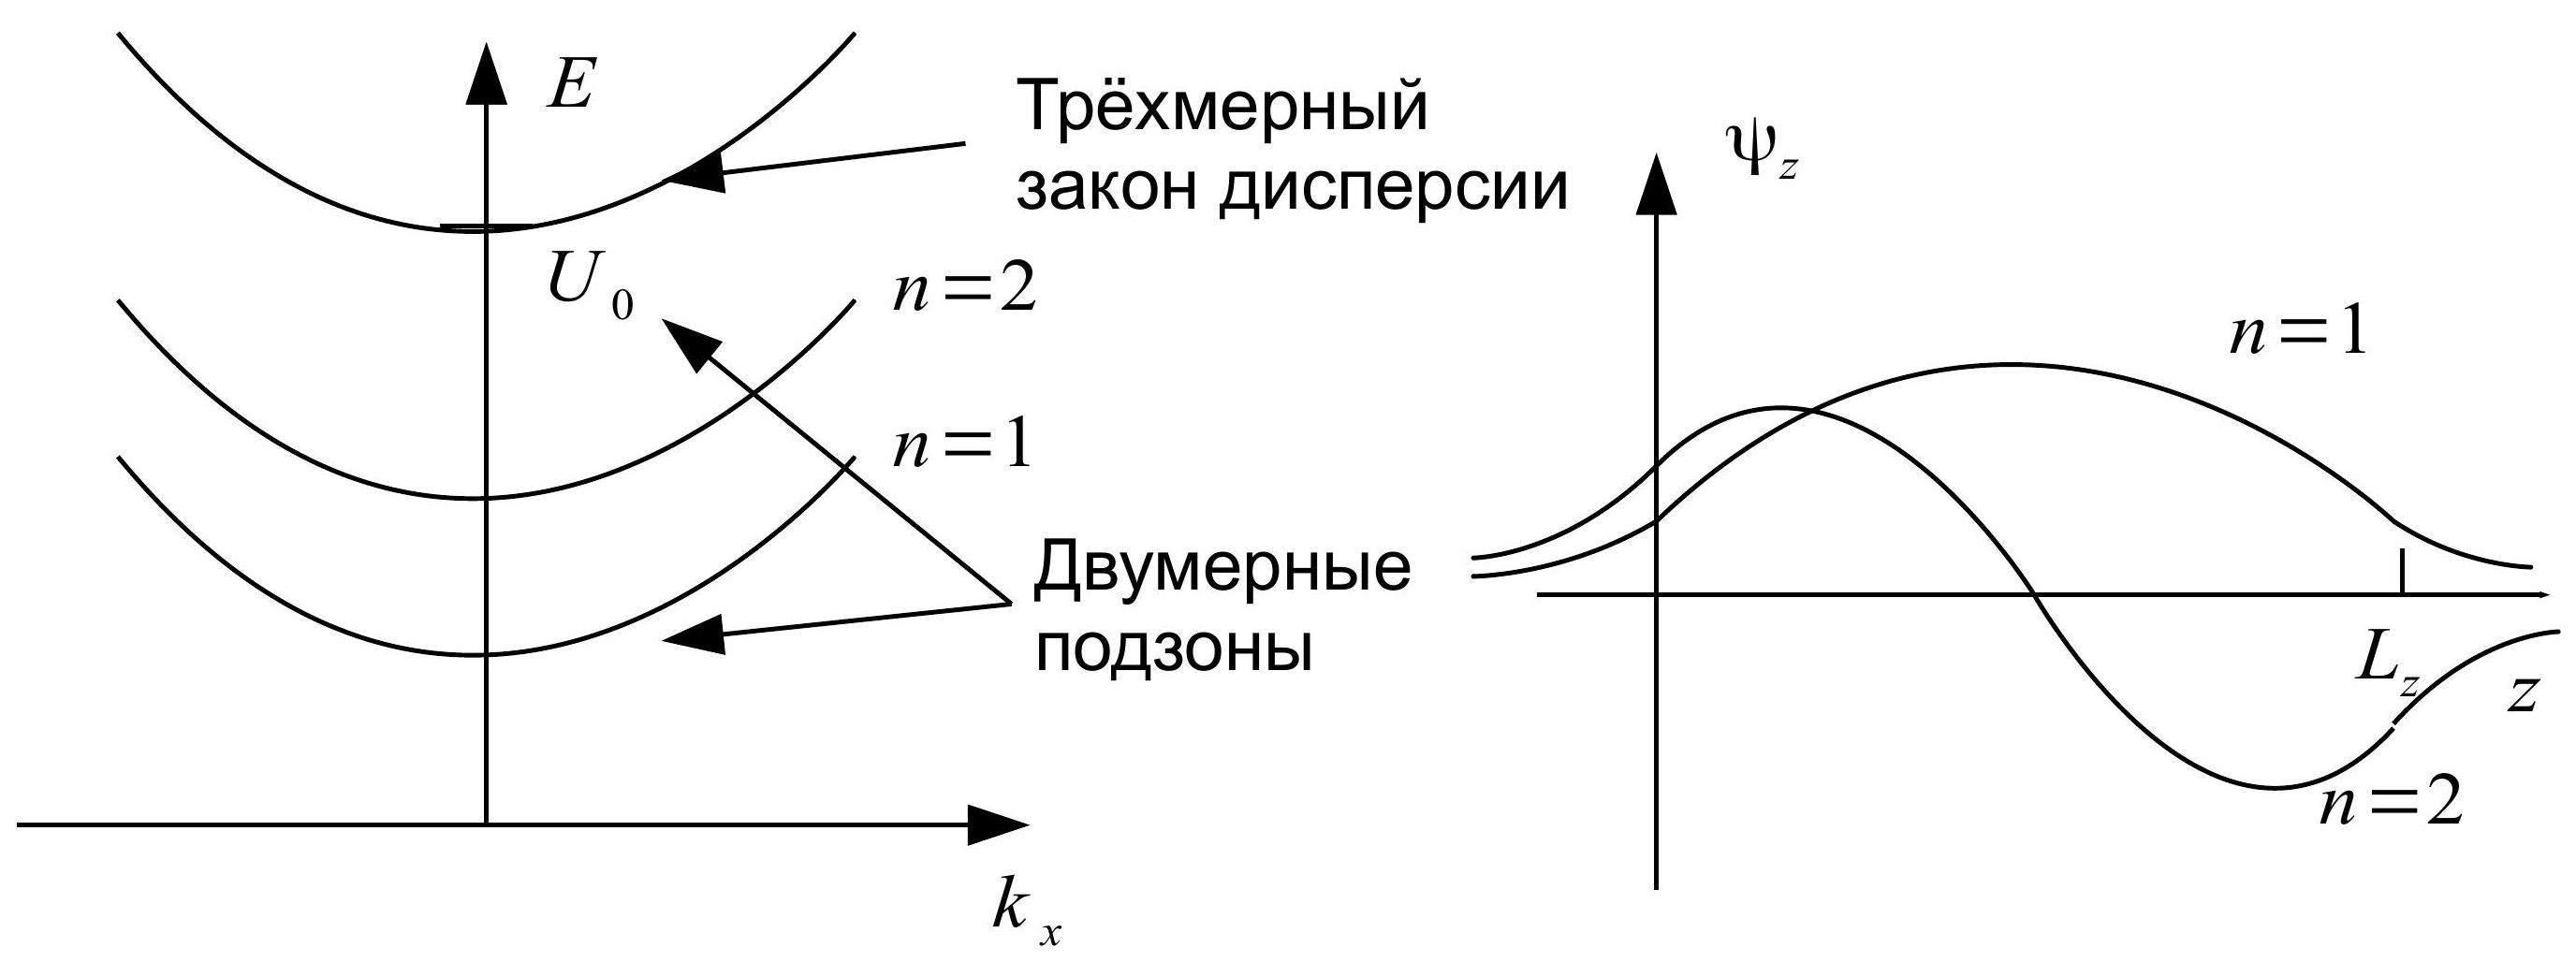
\includegraphics[width=0.7\textwidth]{2023_05_21_66a3dfca5be088b7d6b7g-07}
\end{figure}
 В потенциальном ящике со стенками конечной высоты образуется
конечное число двумерных подзон. Состояния с энергией более
высоты стенок трёхмерные. Волновые функции двумерных состяний
частично проникают в стенки ящика.

\textbf{В реальных двумерных структурах:}
\begin{itemize}
\item Волновые фукции двумерных состояний сосредоточены внутри потенциальной ямы для электронов дырок
\item В двумерной структуре образуется конечное число двумерных подзон.
\itemПри энергии выше потенциального барьера, ограничивающего потенциальную яму существуют трёхмерные состояния
\itemПри наличии потенциальной ямы для дырок образуются двумерные подзоны для дырок
\itemЗакон дисперсии вблизи минимума двумерной подзоны квадратичный, но может быть анизотропным при анизотропии материала структуры

$$
E=E_{n}+\frac{\hbar^{2}}{2}\left(\frac{k_{x}^{2}}{m_{x x}}+\frac{k_{y}^{2}}{m_{y y}}\right), n=1,2,3 \ldots
$$

\itemПри наличии двух типов посителей (например лёгкие и тяжёлые дырки) образуется набор двумерных подзон для носителей каждого типа 

\end{itemize}

\textbf{Энергетический спектр, плотность состояний, концентрация двумерных электронов.}


Квадратичный закон дисперсии:
$$
E(\vec{k})=E_{n}+\frac{\hbar^{2}}{2}\left(\frac{k_{x}^{2}}{m_{x}}+\frac{k_{y}^{2}}{m_{y}}\right)
$$

Плотность состояний

$$
v_{2 D}(E)=\frac{\partial N_{2 D}\left(E^{\prime}<E\right)}{\partial E}
$$

$N_{2 \mathrm{D}}\left(E^{\prime}<E\right)$ - концентрация (на единицу площади) состояний с энергией $E^{\prime}<E$

$$
N_{2 D}\left(E^{\prime}<E\right)=\frac{2}{(2 \pi)^{2}} \sum_{n} S_{n}(E<E)=\frac{2 \cdot 2 \pi \sqrt{\left(m_{x} m_{y}\right)} E}{4 \pi^{2} \hbar^{2}} \sum_{n} \theta\left(E-E_{n}\right)
$$

$S_{n}\left(E^{\prime}<E\right)$ - площадь состояний в простансте квазиволновых векторов, занимаяемая состояниями с энергией $E^{\prime}<E$ в $n$-ой двумерной подзоне
$$
\theta(x)=\left\{\begin{array}{l}
1, x \geq 0 \\
0, x<0
\end{array}\right.
$$

$$
v_{2 D}=\sum_{n} \frac{\sqrt{m_{x} m_{y}}}{\pi \hbar^{2}} \theta\left(E-E_{n}\right)
$$
\begin{figure} [h!]
    \centering
    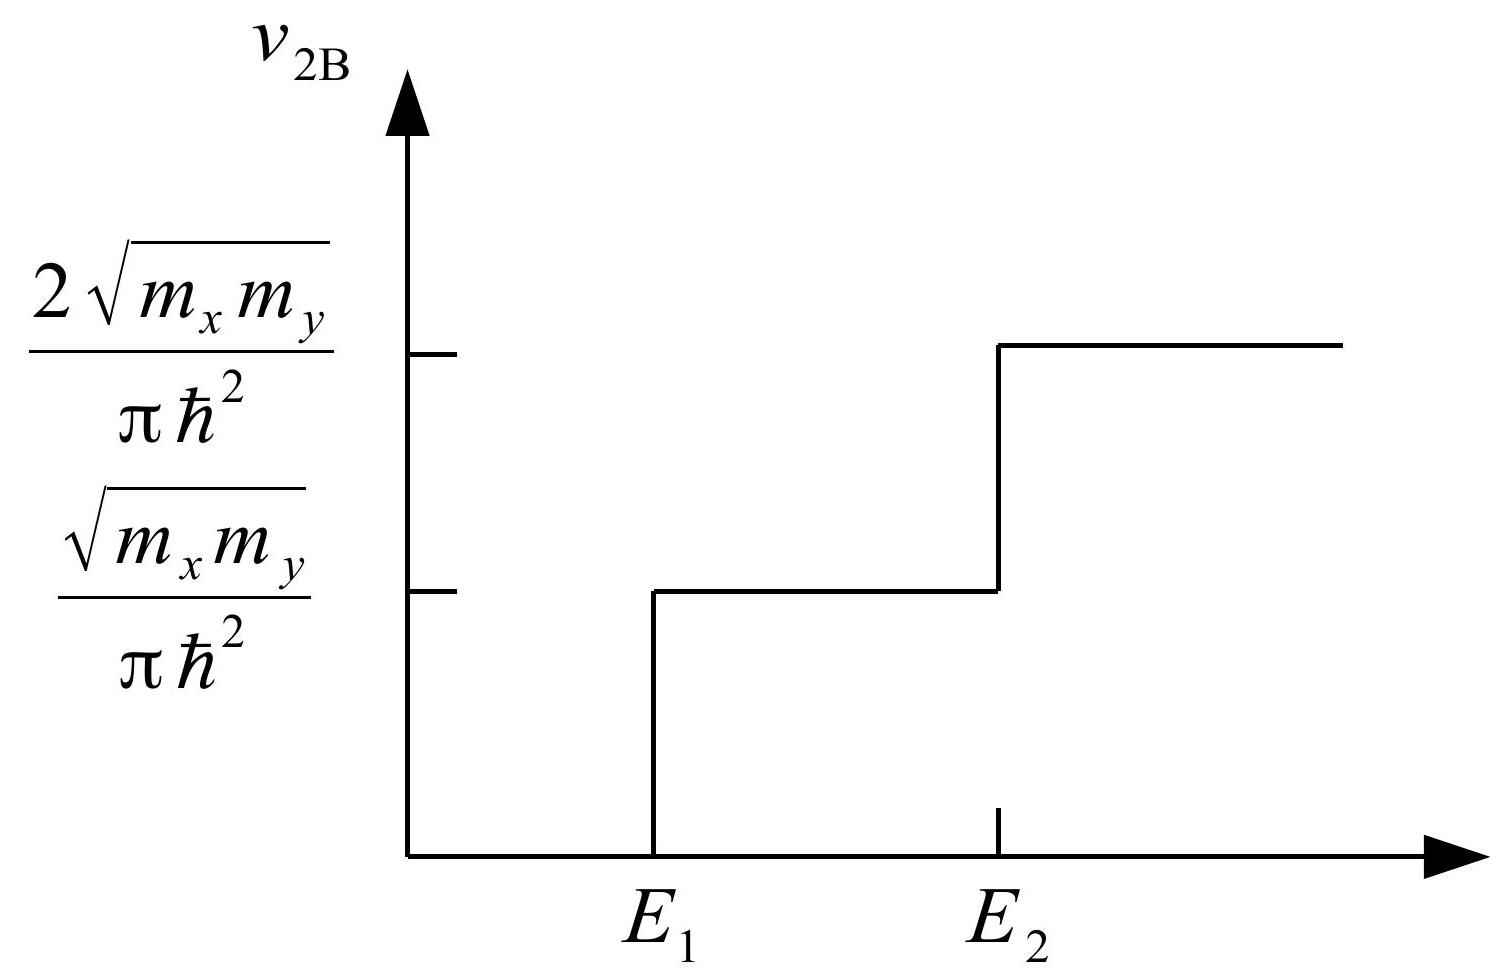
\includegraphics[width=0.7\textwidth]{2023_05_21_66a3dfca5be088b7d6b7g-12}
\end{figure}


Концентрация двумерных электронов:

$$
n_{2 \mathrm{D}}=\int_{-\infty}^{\infty} v_{2 \mathrm{D}}(E) f(E) d E
$$

При $T=0$ (квадратичный закон дисперсии):

$$
n_{2 D}=\sum_{n} \frac{\sqrt{m_{x} m_{y}}}{\pi \hbar^{2}}\left(F-E_{n}\right) \theta\left(F-E_{n}\right)
$$

При T>0 (квадратичный закон дисперсии):

$$
\begin{aligned}
& f(E)=\frac{1}{\exp \left(\frac{E-F}{k_{B} T}\right)+1} \\
& n_{2 D}=\sum_{n} k_{B} T \frac{\sqrt{m_{x} m_{y}}}{\pi \hbar^{2}} \ln \left(1+\exp \left(\frac{F-E_{n}}{k_{B} T}\right)\right)
\end{aligned}
$$
\textbf{Примеры двухмерных структур:}
\begin{itemize}
    \item Структура металл-диэллектрик полупроводник (МДП)
\begin{figure} [h!]
\centering
    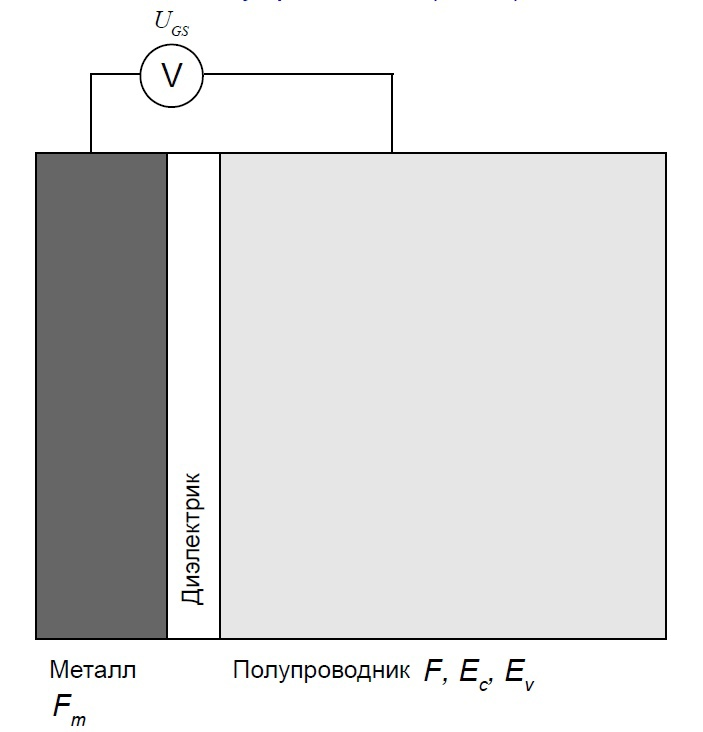
\includegraphics[width=0.4\textwidth]{images/ph28.1.jpg}
    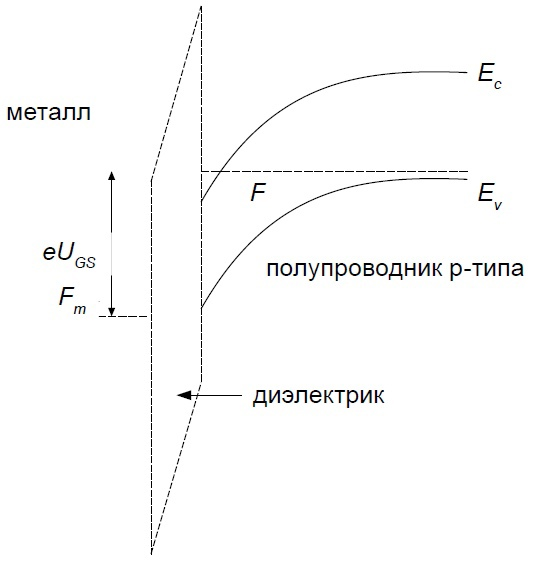
\includegraphics[width=0.4\textwidth]{images/ph28.2.jpg}
    \caption*{Энергетическая диаграмма структуры металл-диэлектрик-
полупроводник (МДП) в режиме инверсии}
\end{figure}
\item Легированные двухмерные структуры
\begin{figure} [h!]
\centering
    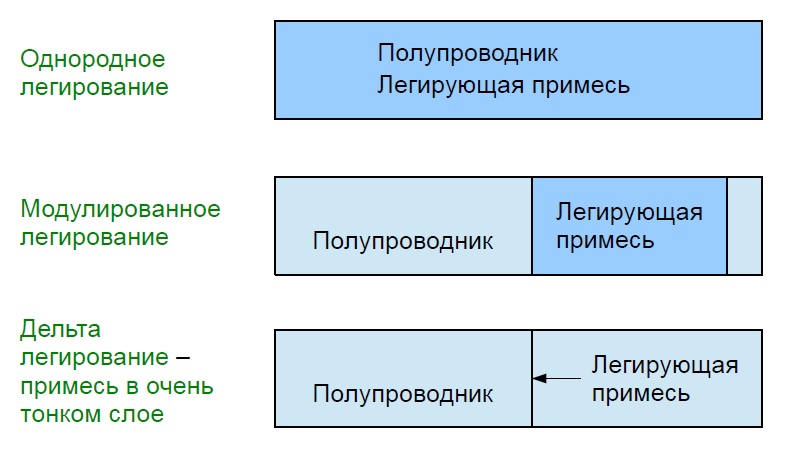
\includegraphics[width=0.7\textwidth]{images/ph28.3.jpg}
\end{figure}
\end{itemize}
\begin{figure} [h!]
\centering
    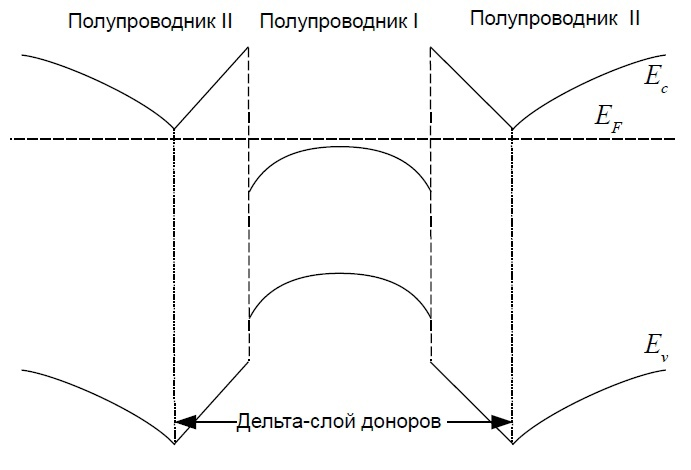
\includegraphics[width=0.7\textwidth]{images/ph28.4.jpg}
\caption*{Энергетическая диаграмма дельта-легированной квантовой ямы. Легирующая примесь отделена от электронов в квантовой яме для
уменьшения их рассеяния и увеличения подвижности.}
\end{figure}

К веществам, имеющим двумерную или квазидвумерную электронную структуру относится графит и его интеркалированные соединения, а также слоистые дихалькогениды переходных металлов и слоистые  полупроводники $\mathrm{A}^{\text {III}}\mathrm{B}^{\text {VI}}$ (пример - InSe).


\section{Целочисленный квантовый эффект Холла. Энергетический спектр и волновые функции электронов в двумерных системах в квантующем магнитном поле. Перенос заряда. Краевые состояния}

Вид сверху двумерной структуры в магнитном поле $B. \quad I-$ сила тока. $U_{x}, U_{y(H)}$ - продольное и поперечное (холловское) напряжение.

\begin{figure}[h!]
    \centering
    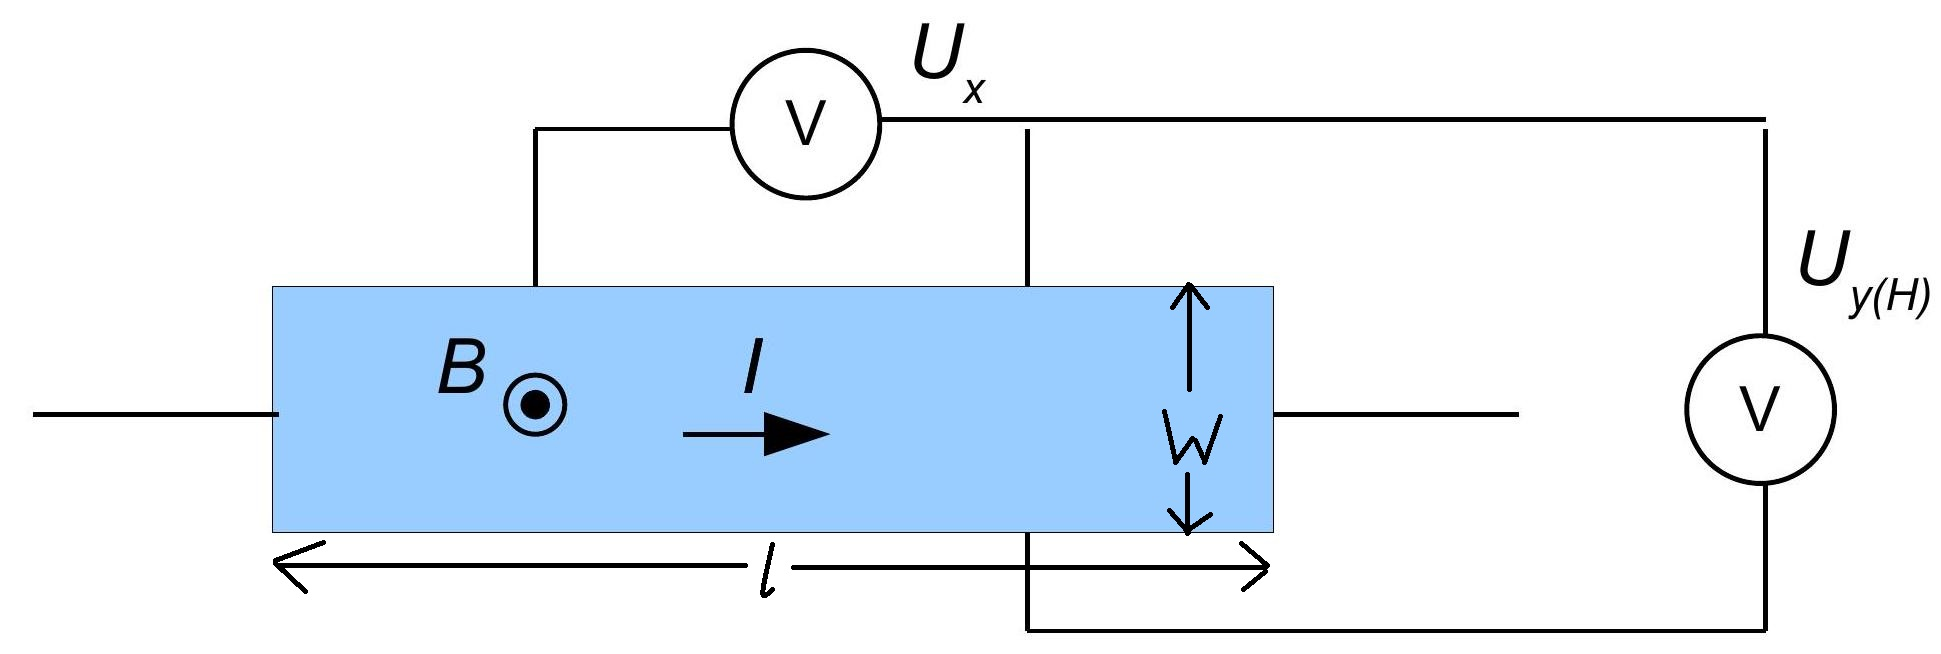
\includegraphics[width=0.7\textwidth]{2023_05_21_c393174d8c3dfa948d89g-01}
\end{figure}

Тензоры электропроводности $\sigma$ и сопротивления $\rho$

$$
\rho=\left\{\begin{array}{cc}
\rho_{x x}=\left(U_{x} / I\right)(w / l) & \rho_{x y}=-U_{y(H)} / I \\
\rho_{y x}=U_{y(H)} / I & \rho_{y y}=\left(U_{y} / I\right)(w / l)
\end{array}\right\} \quad \sigma=\rho^{-1}=\left\{\begin{array}{ll}
\sigma_{x x} & \sigma_{x y} \\
\sigma_{y x} & \sigma_{x x}
\end{array}\right\}
$$


\begin{figure}[h!]
    \centering
    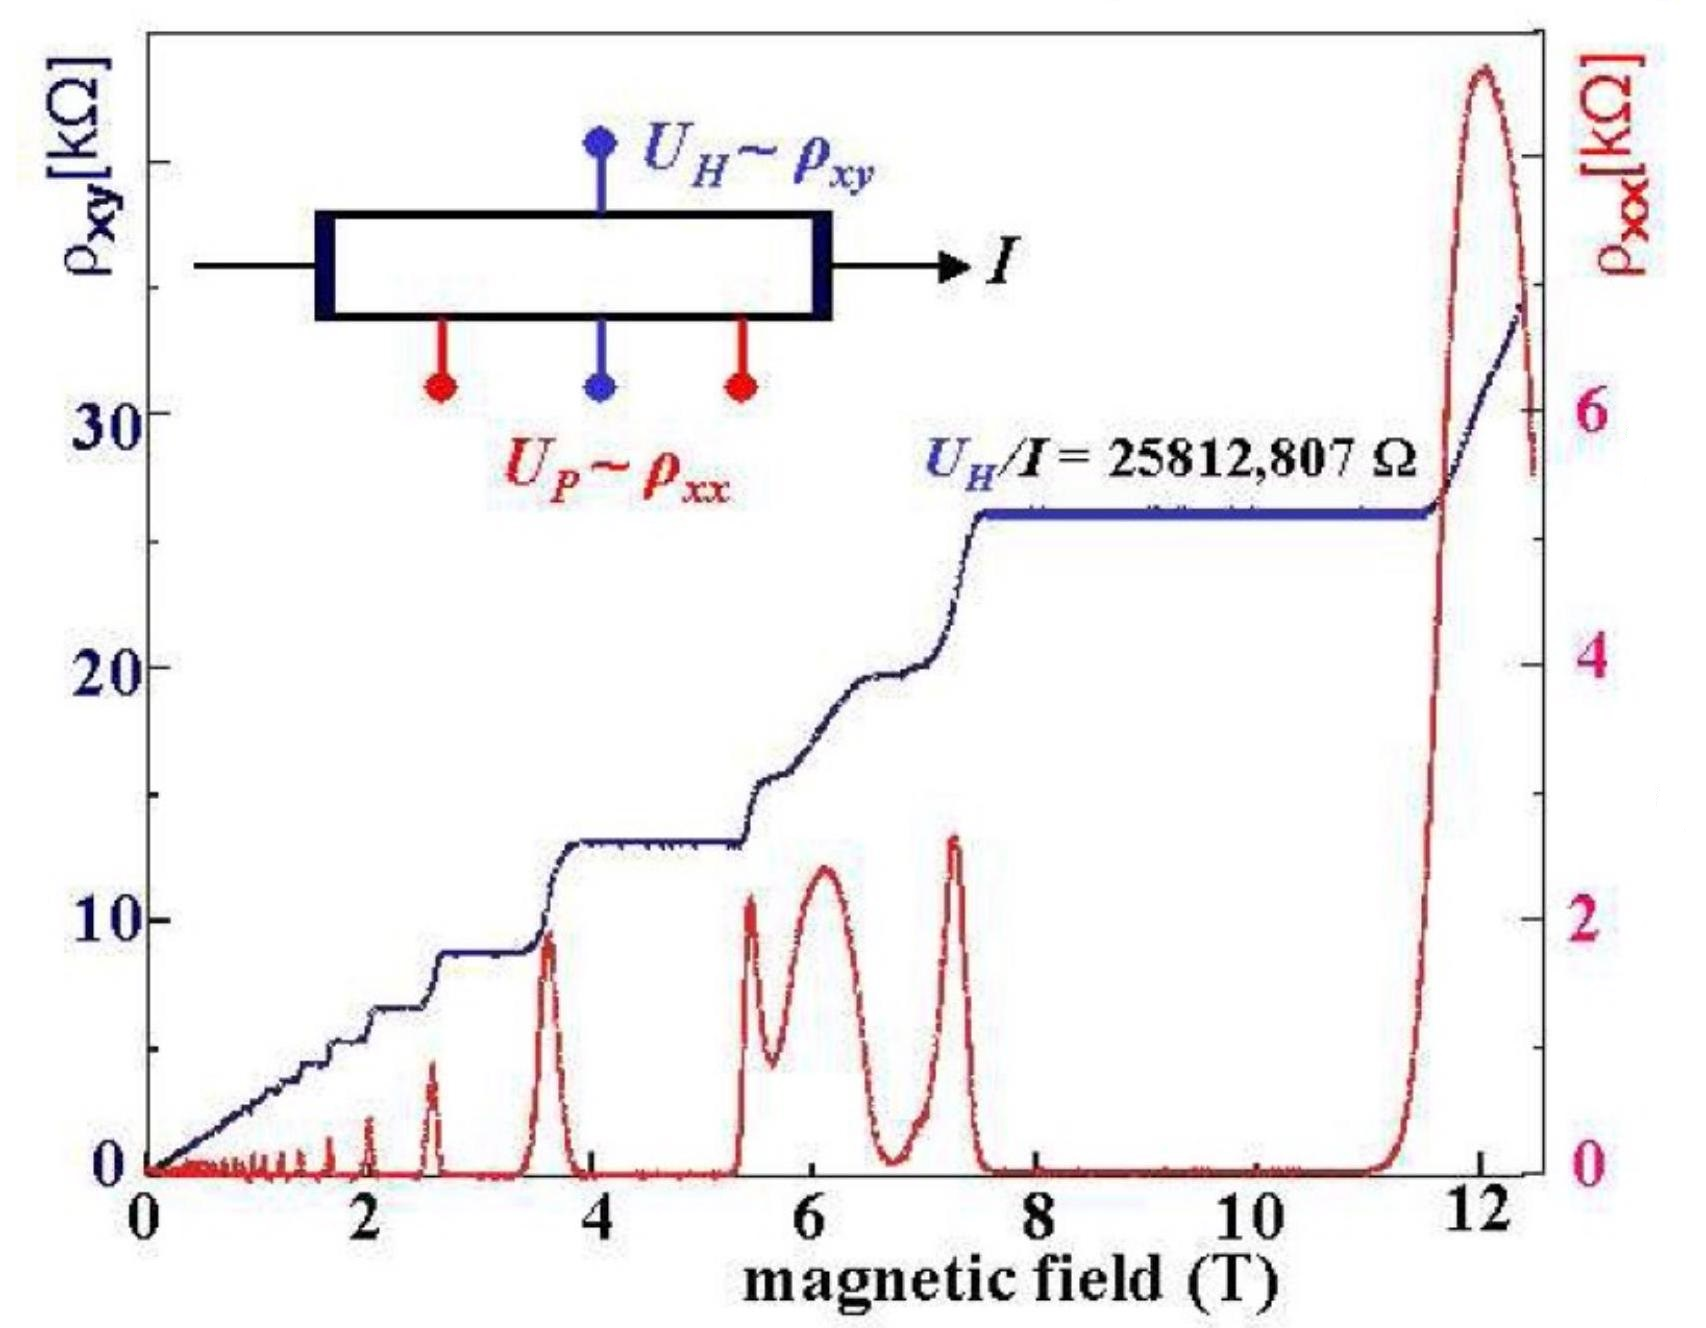
\includegraphics[width=0.7\textwidth]{2023_05_21_c393174d8c3dfa948d89g-02}
    \caption*{Целочисленнный квантовый эффект Холла.}
\end{figure}
При увеличении
напряжения исток-затвор
увеличивается
концентрация двумерных
электронов в структуре.
$\rho_{хх}-$ осциллирует в зависимости от напряжения исток-затвор. В области где $\rho_{x x}$ близко к $0 \rho_{y \times(H)}$ слабо зависит от напряжения (область плато). 
Значение на плато выражается через постоянную Планка и элементарный
заряд: $$
\rho_{y x(H)}=\frac{2 \pi \hbar}{e^2 v}, v=1,2, \ldots
$$
Условие образование уровней Ландау: период классического движения электрона по циклотронной орбите должен быть меньше чем время релаксации импульса, т.е. электрон должен совершить хотя бы один оборот до рассеяния

$$
\omega_{c} \tau \gg 1
$$
Условие на температуру: разность в энергии между уровнями Ландау должно быть больше тепловой энергии
$$
\hbar \omega_{c} \gg k_{B} T
$$
Рассмотрим \textbf{двумерный электрон в сильном магнитном поле:}

обобщённый импульс (квазиимпульс) в магнитном поле
$
\hat{\vec{p}} \rightarrow \hat{\vec{p}}+e \vec{A}
$, 

векторный потенциал (выбирается для прямоугольной структуры): $\vec{A}=(-B y, 0,0)$, 

оператор Гамильтона:$
\hat{H}=\frac{1}{2 m_{e}}(\hat{\vec{p}}+e \hat{\vec{A}})^{2}=\frac{1}{2 m_{e}}\left[\left(\hat{p}_{x}-e B y\right)^{2}+\hat{p}_{y}^{2}\right]
$, 

уравнение Шредингера:$
\hat{H} \psi=E \psi \quad\left(E=E-E_{l}\right) $

В уравнении нет зависимости от координаты х, поэтому волновую функцию можно представить в виде:

$$
\psi(x, y)=\psi_{y}(y) \exp \left(i k_{x} x\right) \quad \hat{p}_{x} \psi(x, y)=\hbar k_{x} \psi_{y}(y) \exp \left(i k_{x} x\right)
$$

В результате уравнение для $\Psi_{y}$ принимает вид:

$$
\begin{gathered}
-\frac{\hbar^{2}}{2 m_{e}}\left(\frac{d^{2} \psi_{y}}{d y^{2}}-\left(\frac{e B y}{\hbar}-k_{x}\right)^{2}\right)=E \psi_{y} \\
\frac{d^{2} \psi_{y}}{d y^{2}}+\frac{e B}{\hbar}\left[2 E \frac{m_{e}}{e \hbar B}-\frac{e B}{\hbar}\left(y-k_{x} \frac{\hbar}{e B}\right)^{2}\right] \psi_{y}=0
\end{gathered}
$$

Граничные условия для $\Psi_{y}$ :
$$
\psi_{y}(y) \rightarrow 0, y \rightarrow \pm \infty
$$
Ведём обозначения:
\begin{itemize}
\item Магнитная длина $l_{B}=\sqrt{\frac{\hbar}{e B}}$
\item Циклотронная энергия $E=\hbar \omega_{c}$
\item Циклотронная частота $\omega_{c}=\frac{e B}{m_{e}}$
\item Безразмерная координата вдоль $\mathrm{Y} \quad \eta=\frac{y-k_{x} l_{B}^{2}}{l_{B}}$
\item Безразмерная Энергия $\quad G=E \frac{m_{e}}{e \hbar B}=\frac{E}{\hbar \omega_{c}}$
\end{itemize}


Получим безразмерное уравнение Шредингера:

$$
\frac{d^{2} \psi_{y}}{d \eta^{2}}+\left(2 G-\eta^{2}\right) \psi_{y}=0
$$

Решение при $\quad \eta=\rightarrow \pm \infty \quad
\frac{d^{2} \psi_{y}}{d \eta^{2}}-\eta^{2} \psi_{y}=0
$

Пусть $\beta=\eta^{2} \quad \Rightarrow
\frac{d^{2} \psi_{y}}{d \eta^{2}}=4 \beta \frac{d^{2} \psi_{y}}{d \beta^{2}}+2 \frac{d \psi_{y}}{d \beta} \rightarrow 4 \beta \frac{d^{2} \psi_{y}}{d \beta^{2}}, \text { при } \beta \rightarrow \infty \quad \Rightarrow
 \frac{d^{2} \psi_{y}}{d \beta^{2}}=\frac{1}{4} \psi_{y}
$

Решение:

$\psi_{y} \rightarrow C \exp \left(-\frac{\beta}{2}\right)=C \exp \left(-\frac{\eta^{2}}{2}\right)$, при $\beta, \eta \rightarrow \infty$

Решение при конечных $\eta$

$$
\psi_{y}=P_{n}(\eta) \exp \left(-\frac{\eta^{2}}{2}\right) \quad P_{n}(\eta)=\sum_{k=0}^{n} a_{n k} \eta^{k}
$$

Уравнение для полинома после подстановки

$$
\frac{d^{2} P_{n}}{d \eta^{2}}-2 \eta \frac{d P_{n}}{d \eta}+(2 G-1) P_{n}=0
$$

Из него получаются уравнения для коэфроициентов полинома

$$
\begin{gathered}
(k+1)(k+2) a_{n 2}+(2 G-1) a_{n 0}=0, k=0,, n \geq 2 \\
(k+1)(k+2) a_{n k+2}-2 k a_{n k}+(2 G-1) a_{n k}=0, \quad 1 \leq k \leq n-2 \\
-2 k a_{n k}+(2 G-1) a_{n k}=0, n-1 \leq k \leq n
\end{gathered}
$$

По условию записи $a_{n n} \neq 0$, поэтому должно быть $-2 n+2 G-1=0 \\ \quad G=n+\frac{1}{2} \text {, а также } a_{n n-1}=0 $

Переходя к исходным переменным, получаем:

Волновая функция:
$$
\psi=\exp \left(i k_{x} x\right) P_{n}\left(\frac{y-k_{x} l_{B}^{2}}{l_{B}}\right) \exp \left[-\frac{\left(y-k_{x} l_{B}^{2}\right)^{2}}{2 l_{B}^{2}}\right]
$$

Энергия (уровни Ландау):

$$
E=E_{n L}=\hbar \frac{e B}{m_{e}}\left(n+\frac{1}{2}\right)=\hbar \omega_{c}\left(n+\frac{1}{2}\right), n=0,1,2 \ldots
$$

При учёте спина электрона к оператору 
Гамильтона добавляется слагаемое $-g \mu_{B} \hat{\vec{B}} \hat{\vec{S}} \Rightarrow$ 
Энергия с учётом спина:
$$
E=E_{n L}=\hbar \frac{e B}{m_{e}}\left(n+\frac{1}{2}\right) \pm \frac{1}{2} g \mu_{B} B \quad \mu_{B}=\frac{e \hbar}{2 m_{0}} 
$$
где g -- фактор Ланде, $m_{0}$ -- масса свободного электрона.

Циклические граничные условия вдоль $X: \psi\left(x+L_{x}\right)=\psi(x)$
Это накладывет условия на $k_{x}$:
$$ k_{x}=\frac{2 \pi}{L_{x}} n_{x}, n_{x}=0, \pm 1, \pm 2, \ldots $$

При изменении $n_{x}$ на 1 волновая функция смещается на
$
\Delta y=\Delta k_{x} l_{B}^{2}=\frac{2 \pi \hbar}{e B L_{x}}
$ -- это размер волновой фуунции вдоль оси $Y$.

Если размер структуры вдоль оси $Y$ равен $L_{y}$, Количество состояний для уровня Ландау
$$
N_{L}=\frac{L_{y}}{\Delta y}=\frac{L_{y}}{\Delta k_{x} l_{B}^{2}}=L_{x} L_{y} \frac{e B}{2 \pi \hbar}
$$
Или на единицу площади двумерной структуры
$$
N_{L}=\frac{e B}{2 \pi \hbar}=\frac{1}{2 \pi l_{B}^{2}}
$$

\begin{figure}[h!]
    \centering
    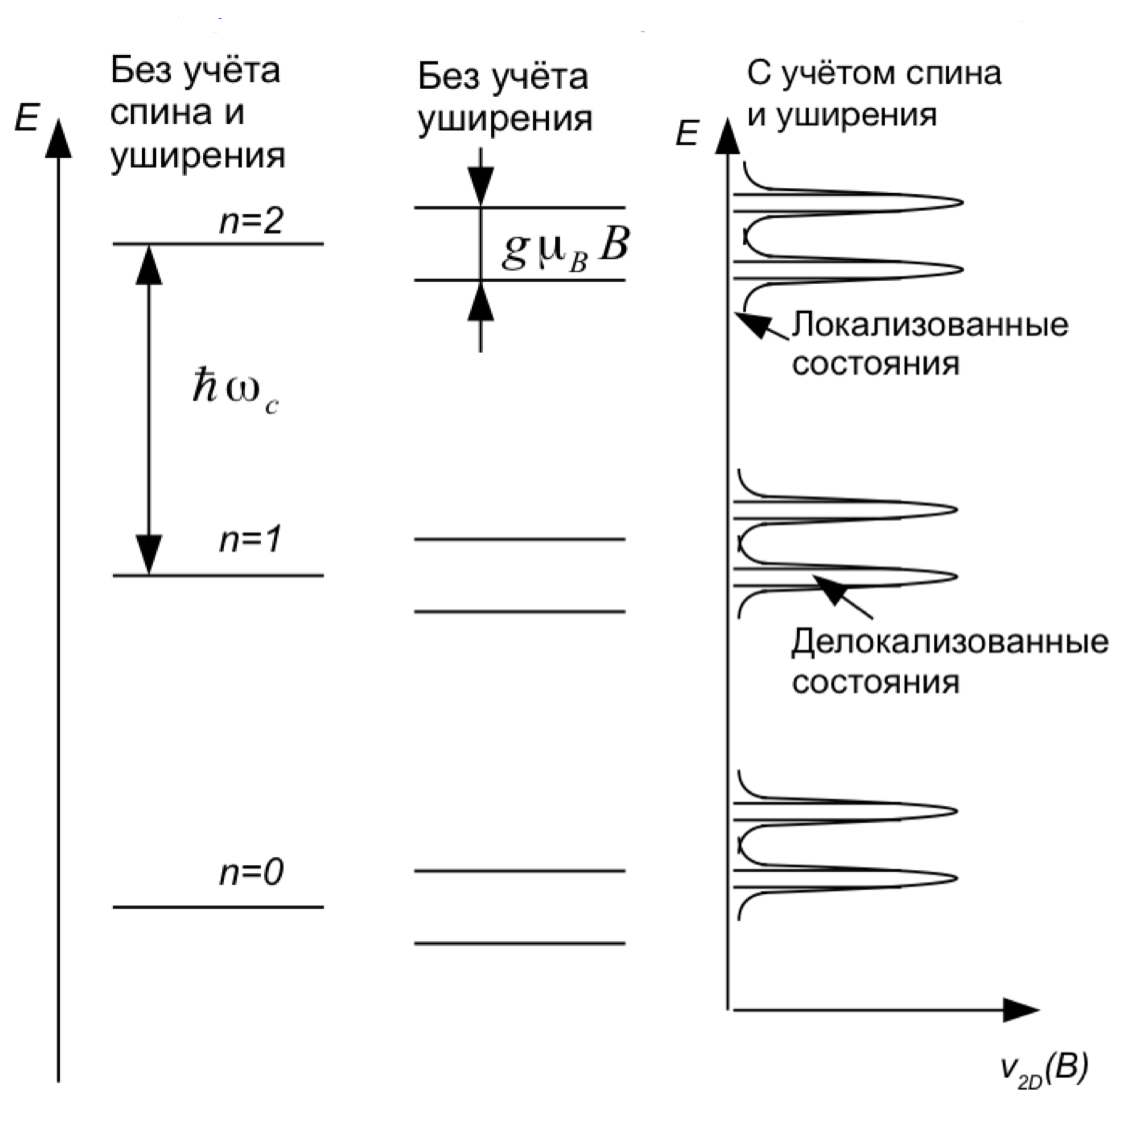
\includegraphics[width=0.8\textwidth]{images/ph29.jpg}
    \caption*{Энергетический спектр электронов в магнитном поле. (Из-за спина уровни Ландау расшепляются, из-за беспорядка уширяются)}
\end{figure}

\begin{figure}[h!]
    \centering
    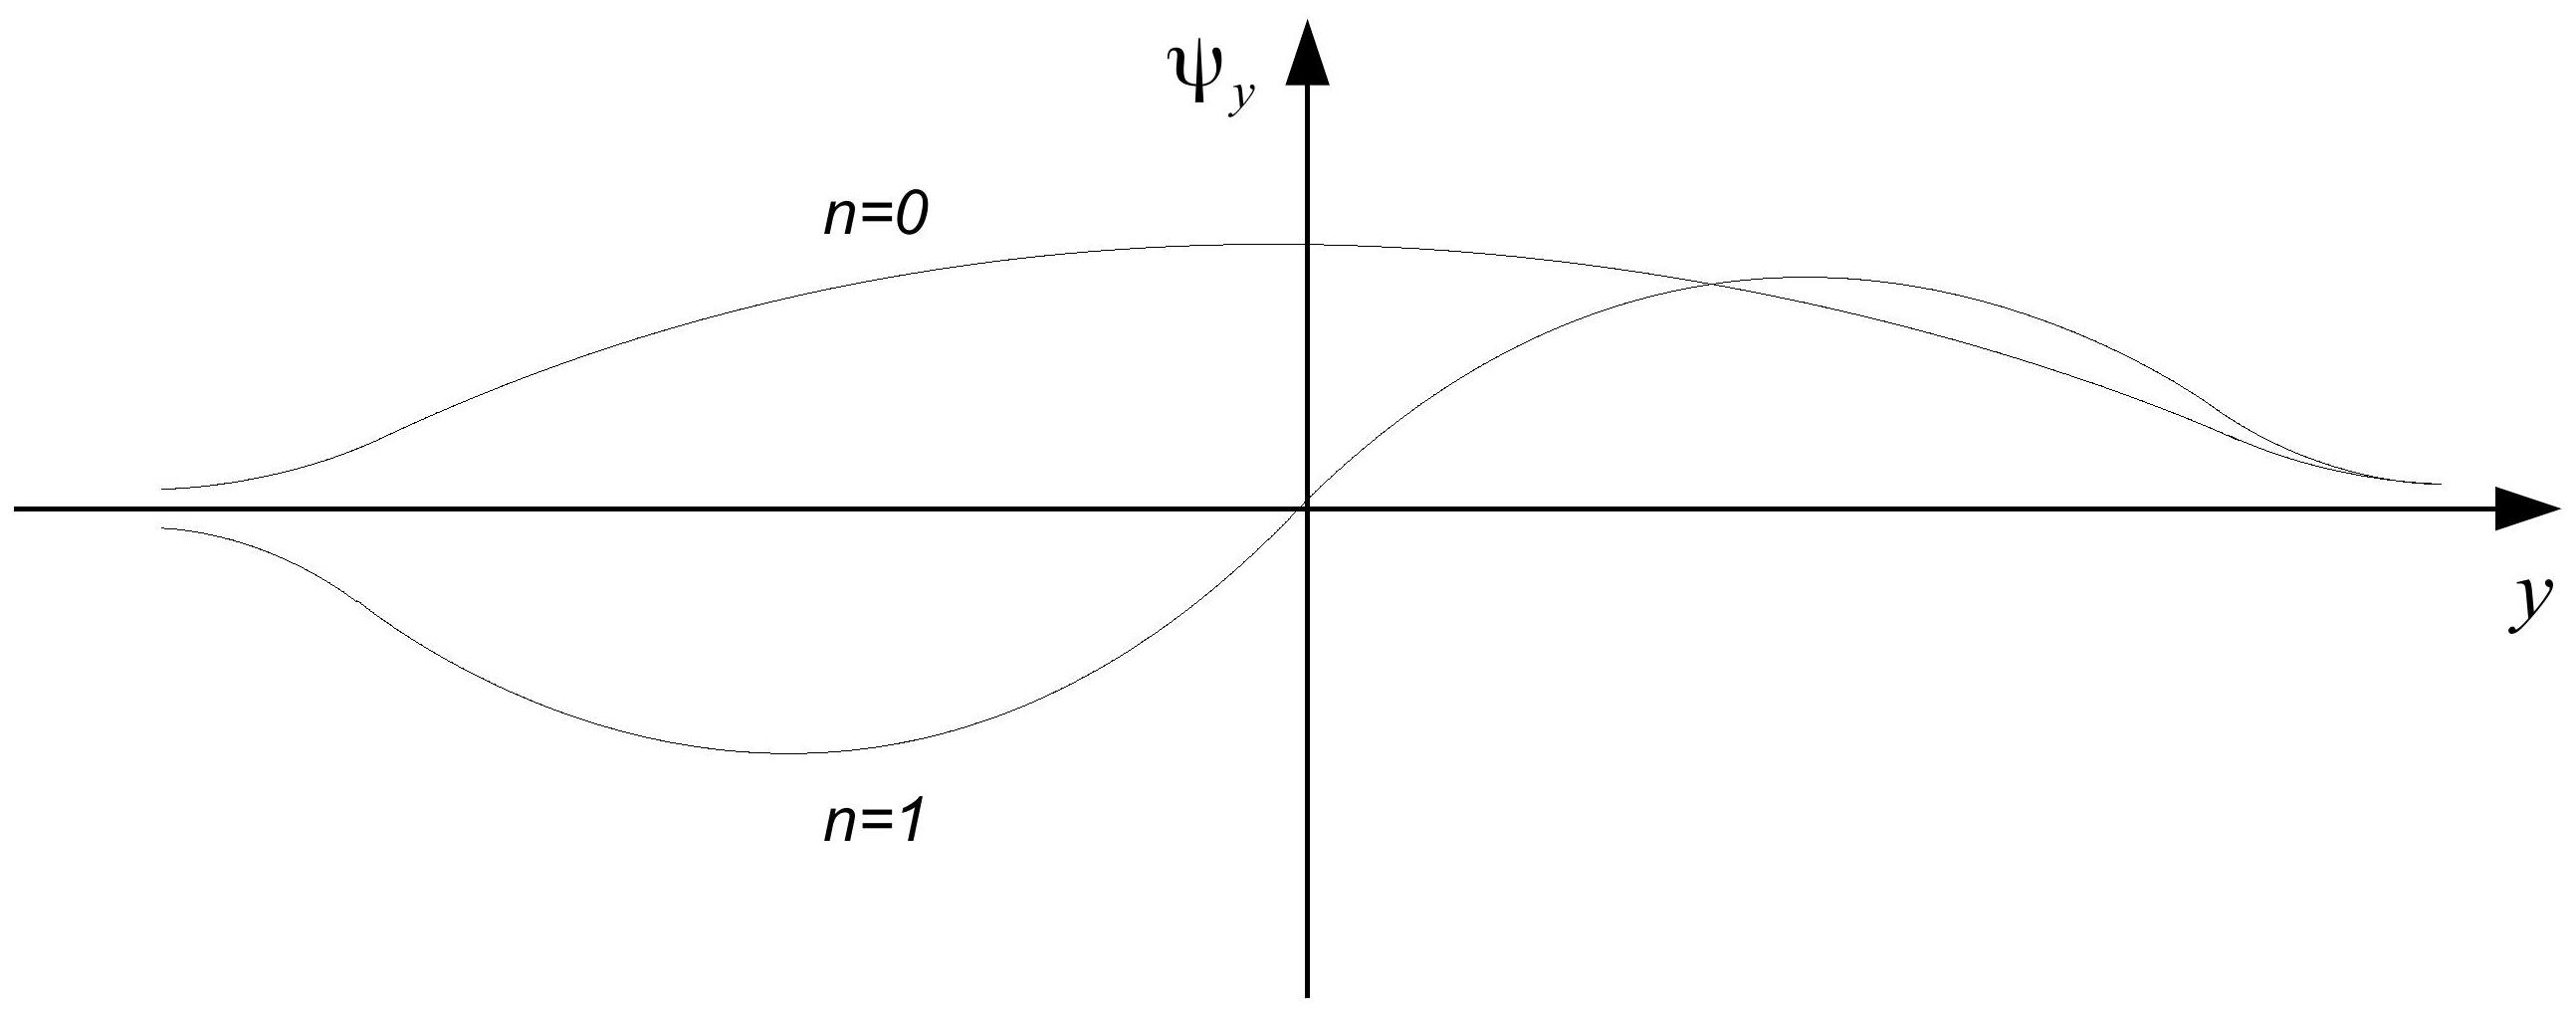
\includegraphics[width=0.8\textwidth]{2023_05_21_c393174d8c3dfa948d89g-11}
    \caption*{Зависимость волновой функции от у}
\end{figure}

Центр волновой фрункции в направлении у
$
\int_{-\infty}^{\infty}\left|\psi_{y}(y)\right|^{2} y d y=k_{x} l_{B}^{2}
$


\textbf{Перенос заряда:}

Вычислим полную силу тока через плотность потока вероятности:
Для одного состояния сила тока
$$
I_1=-e \int_{-\infty}^{\infty} i_x(y) d y
$$
Полная сила тока
$$
I(B)=\int_{-\infty}^{\infty} I_1(E) v_{2 \mathrm{D}}(B) f(E) d E
$$
Подставляем полученную волновую функцию
$$
I_1=-\frac{e^2 B}{2 m_e}\left(k_x l_B^2-\int_{-\infty}^{\infty} y|\psi(y)|^2 d y\right)=0
$$
Как переносится ток в магнитном поле? В эксперименте ток не нулевой.


При Т $\approx 0$ (КЭХ наблюдается при низкой температуре) можно выделить два случая в зависимости от расположения уровня Ферми.

\textit{1. Уровень Ферми в области энергий делокализованных состояний.}

\begin{figure}[h!]
    \centering
    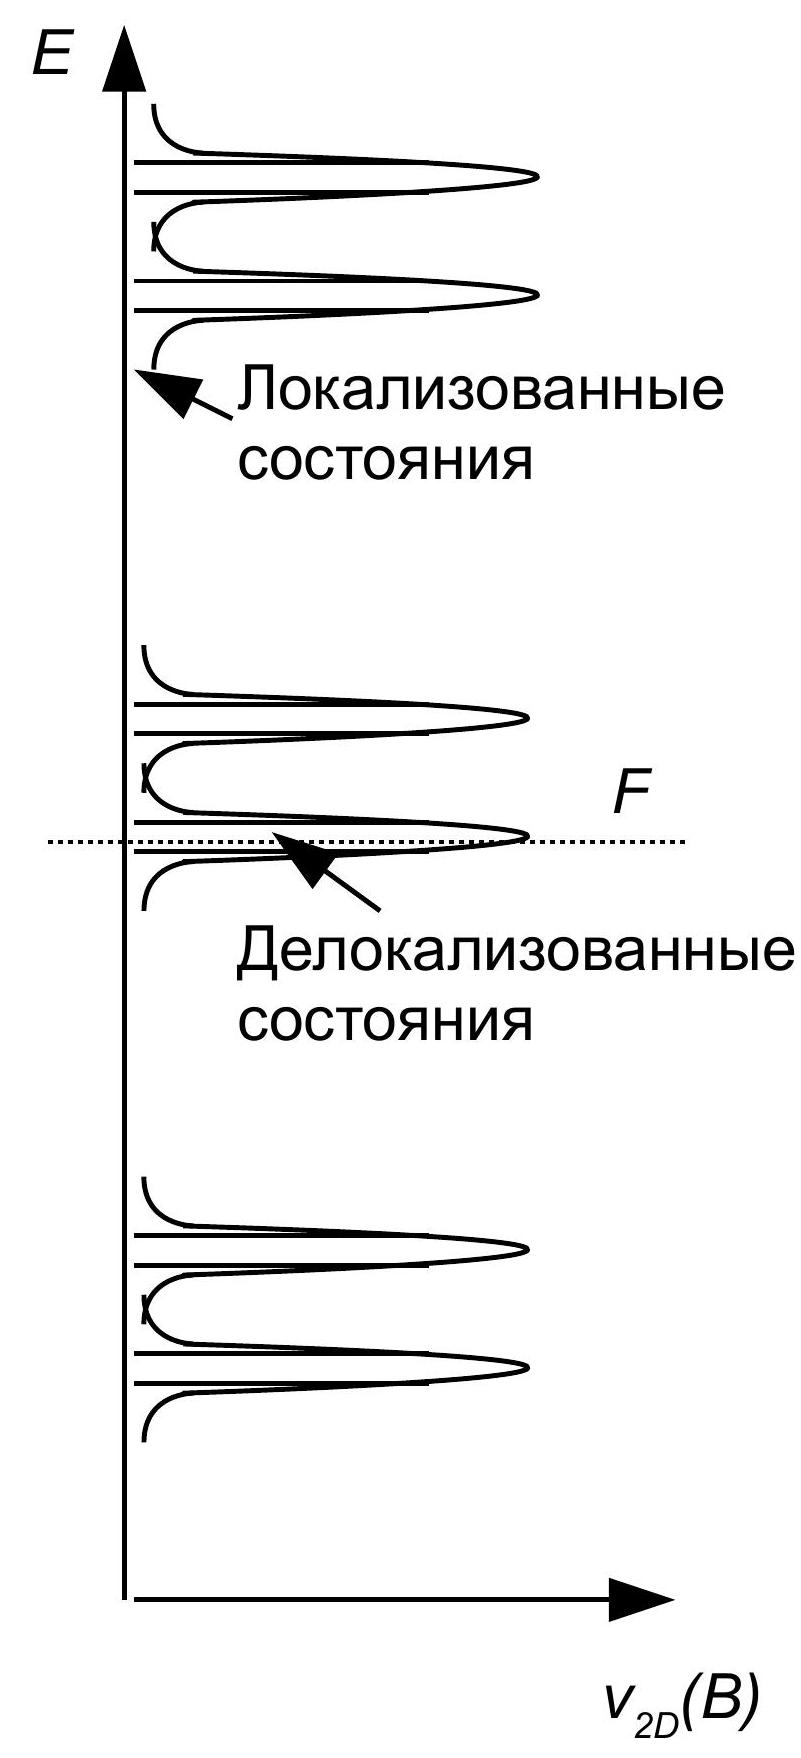
\includegraphics[width=0.3\textwidth]{2023_05_21_c393174d8c3dfa948d89g-14(2)}
\end{figure}

Электрическое поле $E_{x}$ уменьшает $k_{x}$ на $-e E_{x} \tau / \hbar$ В результате при меньших у состояния заполняются электронами с большей вероятностью. Нарушается
электронейтральность структуры, появляется компенсирующее электрическое поле вдоль оси Y и напряжение Холла

\begin{figure}[h!]
    \centering
    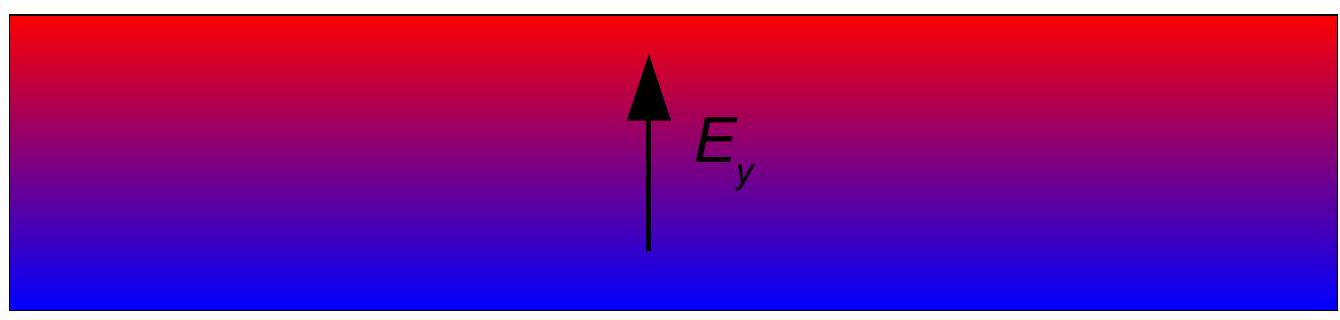
\includegraphics[width=0.3\textwidth]{2023_05_21_c393174d8c3dfa948d89g-14(1)}
\end{figure}

Электрическое поле $E_{y}$ искажает волновую функцию, так что её центр смещается в сторону больших $Y$ от $k_{x} I_{B}^{2}$. Поэтому сила тока одного состояния становится отличной от 0.
\begin{figure}[h!]
    \centering
    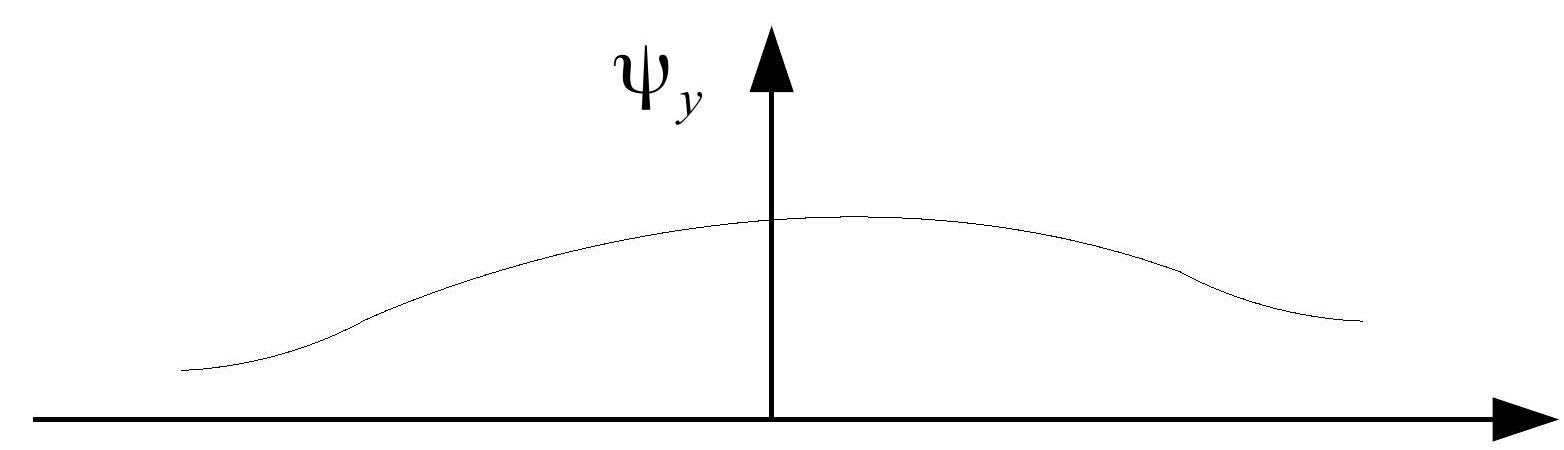
\includegraphics[width=0.6\textwidth]{2023_05_21_c393174d8c3dfa948d89g-14}
\end{figure}


\textit{2. Уровень Ферми в области энергий локализованных состояний.}

В этом случае перераспределение электронов между
делокализованными состояниями невозможно. На краях
структуры потенциальная энергия электронов увеличивается. Уровни Ландау загибаются вверх и пересекают уровень Ферми. В местах пересечения образуются одномерные токонесущие состояния шириной порядка $I_B$ --- краевые состояния.
\begin{figure}[h!]
    \centering
    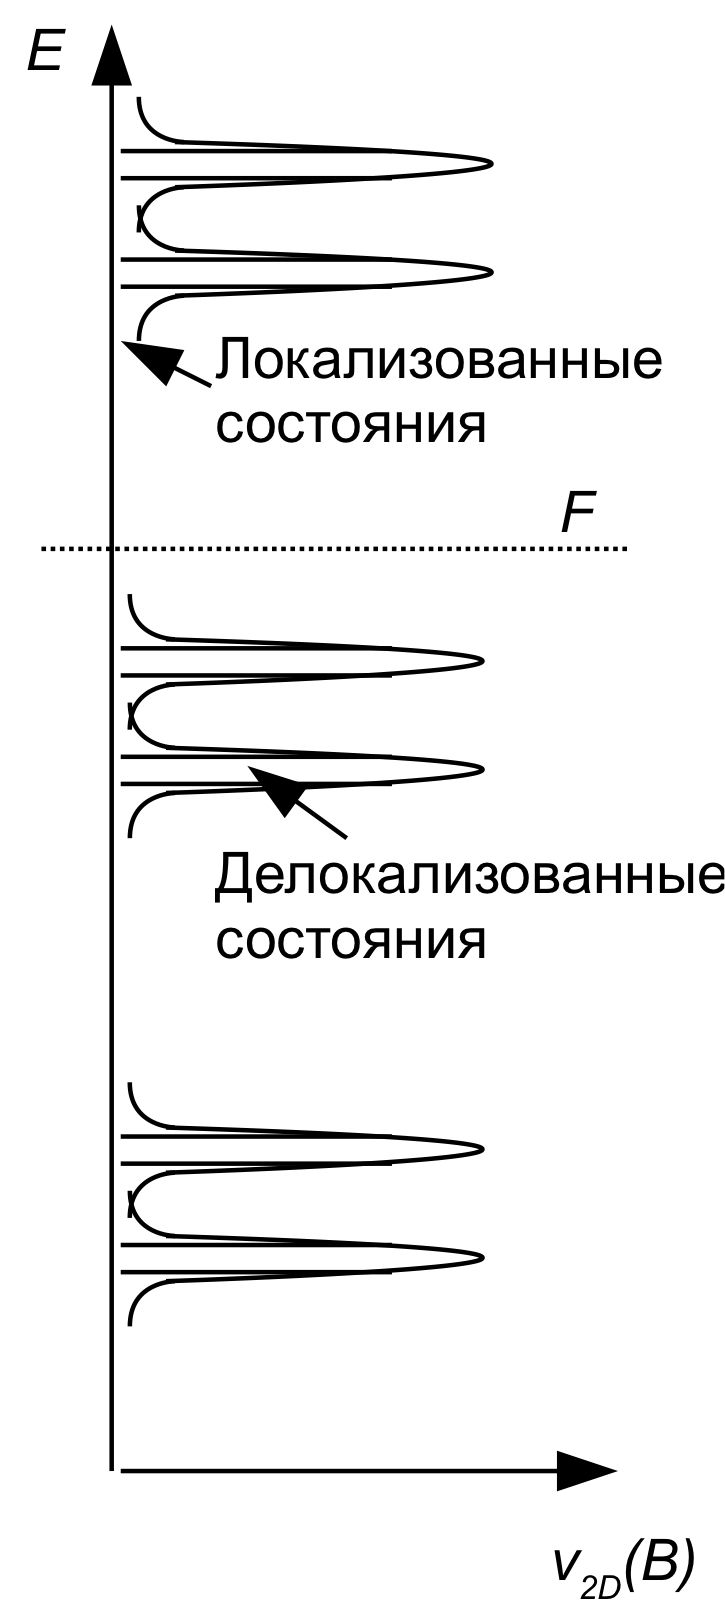
\includegraphics[width=0.3\textwidth]{images/ph29.2.jpg}
\end{figure}
\begin{figure}[h!]
    \centering
    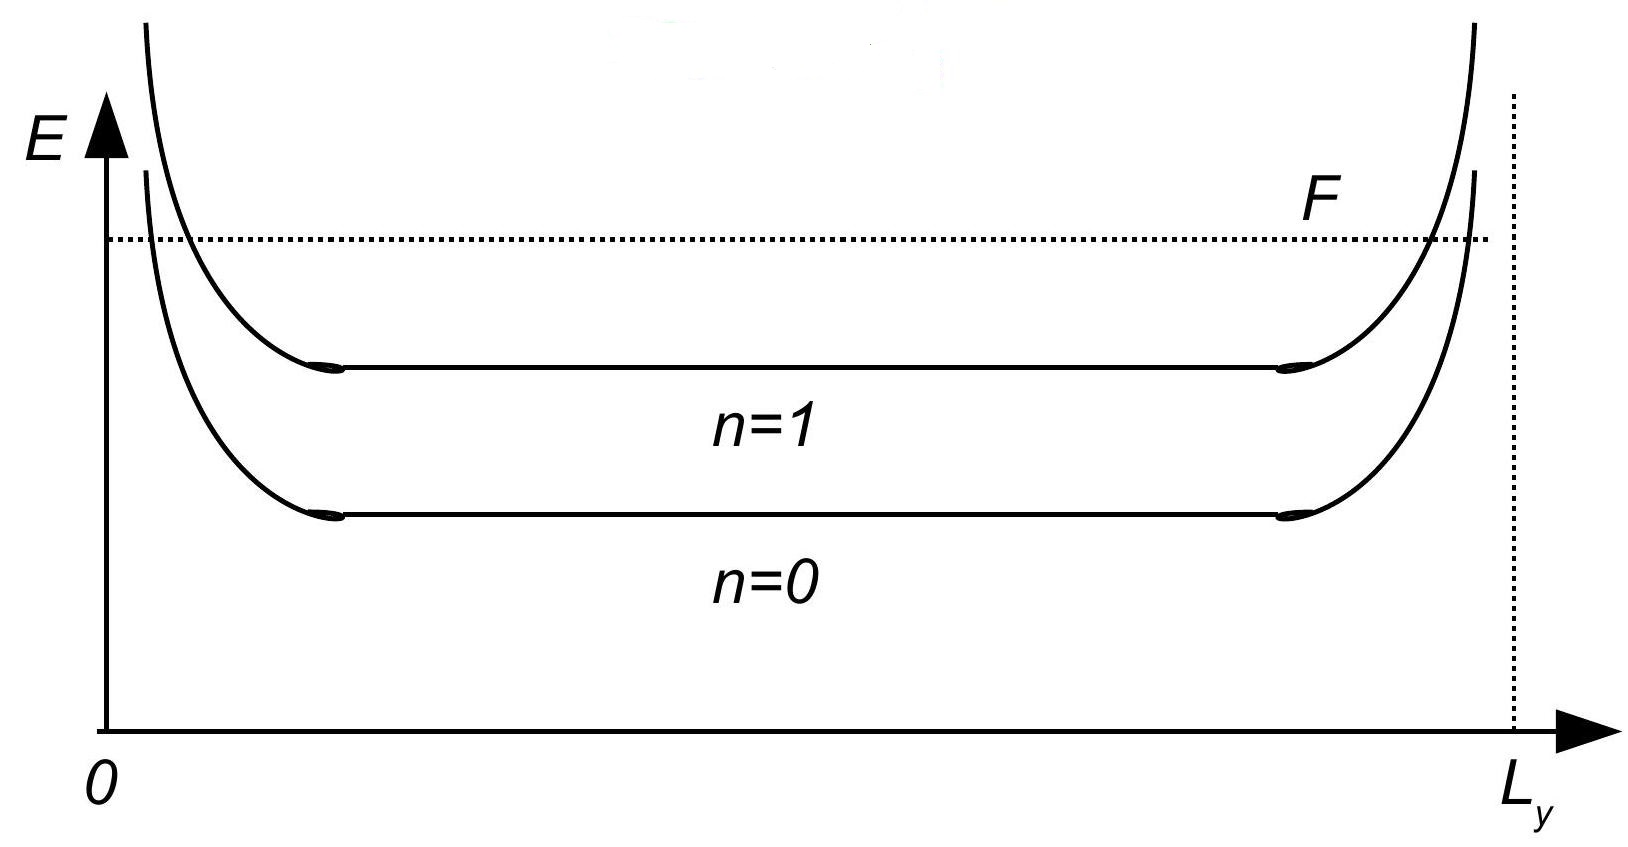
\includegraphics[width=0.6\textwidth]{2023_05_21_c393174d8c3dfa948d89g-15(2)}
\end{figure}

Направление движения электронов в этих состояниях задано отклонением центра волновой функции от $k_{x} I_{B}{ }^{2}$. Это отклонение для противоположных краёв
противоположное. Поэтому ток в одномерных каналах слева и справа течёт в разных направлениях. 

\textbf{Сила тока переносимого краевыми состояниями образованными от одного уровня Ландау ( $T=0 \mathrm{~K})$.}:

Время релаксации $\tau$ и плотность состояний зависят от энергии. Поэтому при поддержании постоянной силе тока напряжение вдоль оси Х осциллирует при пересечении уровнем Ферми уровня Ландау.
Эти осцилляции периодичны в зависимости от $1 / B$
Запишем условие совпадения уровня Ферми с уровнем Ландау с номером $n$ и $n+1$
$$
F-E_l=\frac{\hbar e B_n}{m_e}\left(n+\frac{1}{2}\right) \quad F-E_l=\frac{\hbar e B_{n+1}}{m_e}\left(n+1+\frac{1}{2}\right)
$$
Отсюда получаем
$$
n+\frac{1}{2}=\frac{m_e\left(F-E_l\right)}{\hbar e B_n} \quad n+1+\frac{1}{2}=\frac{m_e\left(F-E_l\right)}{\hbar e B_{n+1}}
$$
Вычитаем из правого левое и получаем для периода $T_B$ и частоты $F_B$ осцилляций от двумерной подзоны с минимумом энергии $E_1$.
$$
T_B=\frac{1}{B_{n+1}}-\frac{1}{B_n}=\frac{e \hbar}{m_e\left(F-E_l\right)} \quad F_B=\frac{1}{T_B}=\frac{m_e\left(F-E_l\right)}{e \hbar}
$$

Сила тока переносимого левым краевым состоянием $(y=0)$
$$
I_{+}=\frac{e}{2 \pi} \int_{E_{n L}}^{F_{l}} v_{x} d k_{x}=\frac{e}{2 \pi \hbar} \int_{E_{n L}}^{F_{l}} \frac{d E}{d k_{x}} d k_{x}=\frac{e}{2 \pi \hbar}\left(F_{l}-E_{n L}\right)
$$

Сила тока переносимого правым краевым состоянием $\left(y=L_{y}\right)$

$$
I_{-}=\frac{e}{2 \pi} \int_{E_{n L}}^{F_{r}} v_{x} d k_{x}=\frac{e}{2 \pi \hbar} \int_{E_{n L}}^{F_{r}} \frac{d E}{d k_{x}} d k_{x}=\frac{e}{2 \pi \hbar}\left(F_{r}-F_{n l}\right)
$$

Полная сила тока

$$
I=I_{+}-I_{-}=\frac{e}{2 \pi \hbar}\left(F_{l}-F_{r}\right)=\frac{e^{2}}{2 \pi \hbar} U_{H}
$$

В случае если v уровней Ландау расположено ниже уровня Ферми

$$
I=\frac{e^{2} v}{2 \pi \hbar} U_{H}
$$

$F_{p} F_{r}-$ уровень Ферми с левого и правого края







\section{Сверхрешетки. Энергетический спектр электронов, минизоны. Проводимость вдоль и перпендикулярно оси сверхрешётки. Осцилляци Блоха. Отрицательная дифференциальная проводимость. Резонансное туннелирование}


\textbf{Полупроводниковые сверхрешётки:}


Сверхрешётка (СВР) – структура, в которой имеется исскуственное
периодическое изменение свойств.


Классификация по размерности:
\begin{itemize}
    \item Одномерная СВР --– периодическое изменение свойств в одном направлении.
    \item Двумерная СВР --– периодическое изменение свойств в двух направлениях
    \item Трёхмерная СВР --– периодическое изменение свойств в трёх направлениях (искуственный кристалл)
\end{itemize}


Композиционные СВР –-- периодичночть обеспечивается периодическим изменением химического состава:
\begin{itemize}
    \item Композиционные СВР типа I –-- чередование слоёв разных
полупроводников, причём запрещённая зона одного полупроводника
расположена в пределах запрещённой зоны второго полупроводника.
\begin{figure}[h!]
    \centering
    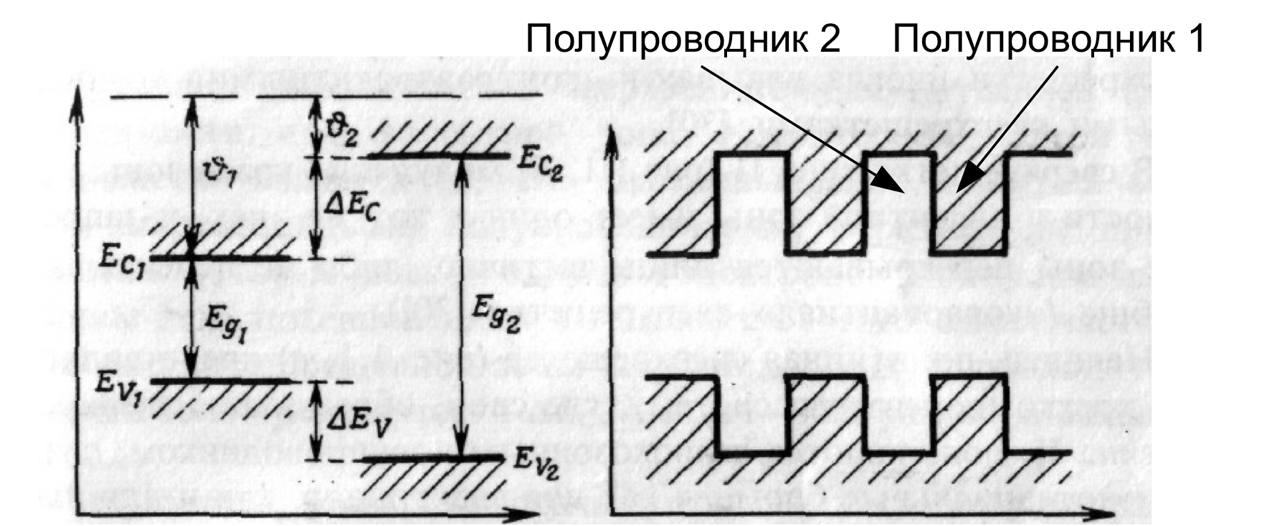
\includegraphics[width=0.5\textwidth]{images/ph30.1.jpg}
\end{figure}
Примеры: $\quad\left(\mathrm{Al}_{\mathrm{x}} \mathrm{Ga}_{1-\mathrm{x}} \mathrm{As} / \mathrm{GaAs}\right)_{\mathrm{n}}, \quad\left(\mathrm{GaAs} / \mathrm{In}_{\mathrm{x}} \mathrm{Ga}_{1-\mathrm{x}} \mathrm{As}\right)_{\mathrm{n}}, \quad\left(\mathrm{GaP} / \mathrm{GaAs}_{\mathrm{x}} \mathrm{P}_{1-\mathrm{x}}\right)_{\mathrm{n}}, \quad(\mathrm{ZnS} / \mathrm{ZnSe})_n$ $(\mathrm{HgTe} / \mathrm{CdTe})_x,\left(\mathrm{Si} / \mathrm{Si}_{1-\mathrm{x}} \mathrm{Ge}_{\mathrm{x}}\right)_n$
    \item Композиционные СВР типа II –-- чередование слоёв разных полупроводников, причём запрещённая зона каждого полупроводника выходит за пределы запрещённой зоны другого полупроводника частично или полностью.
\begin{figure}[h!]
    \centering
    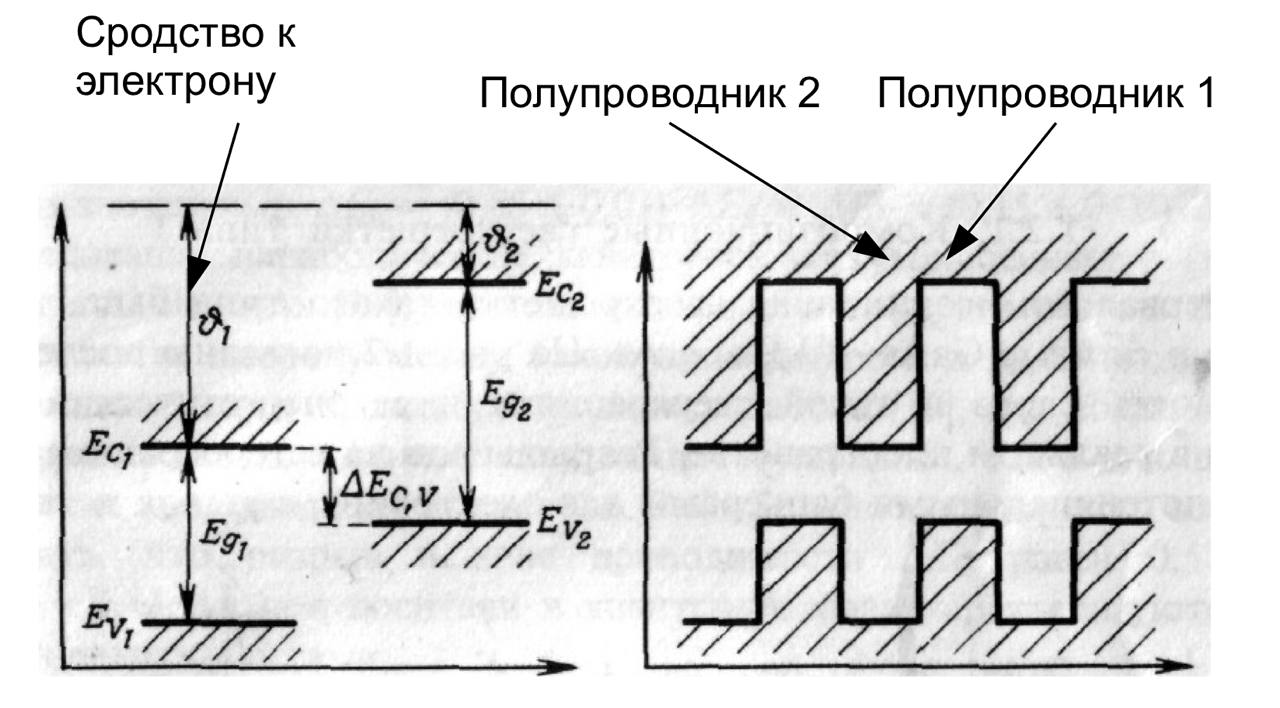
\includegraphics[width=0.5\textwidth]{images/ph30.2.jpg}
\end{figure}
Пример материалов для слоёв: 

1) Полупроводник 1: $\mathrm{GaSb}_{1-y} \mathrm{As}_{\mathrm{y}}$ Полупроводник 2: $\ln _{1-x} \mathrm{Ga}_x \mathrm{As}$

2) Полупроводник 1: $\mathrm{Pb}_{1-\mathrm{y}} \mathrm{Sn}_{\mathrm{y}} \mathrm{Te}$ Полупроводник 2: $\mathrm{Pb}_{1-\mathrm{x}} \mathrm{Sn}_{\mathrm{x}} \mathrm{Te}(\mathrm{x} \neq \mathrm{y})$    

\item Политипные композиционные СВР.
    \begin{figure}[h!]
    \centering
    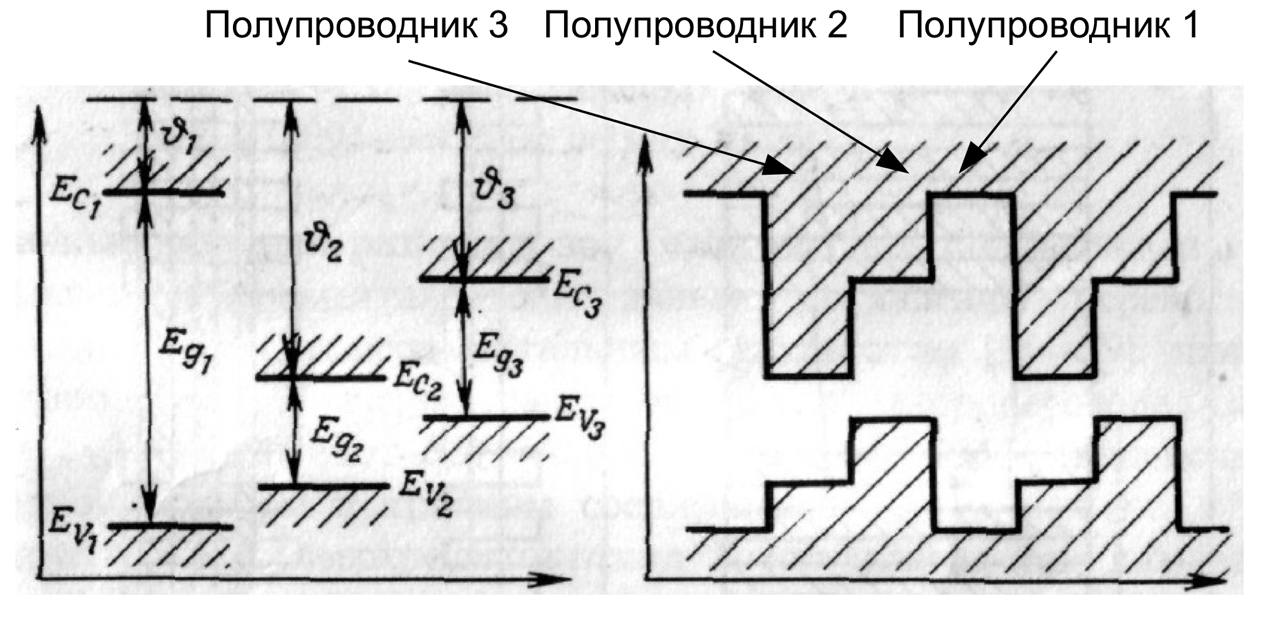
\includegraphics[width=0.5\textwidth]{images/ph30.3.jpg}
    \end{figure}

 Пример: $(AlSb/GaSb/InAs)_n$ 
\end{itemize}


Легированные СВР –-- СВР, в которых периодически изменяется
содержание легирующей примеси, что обеспечивает например,
периодическое чередование слоёв n- и p-типа.

Легированные композитные СВР --– композитные СВР, в которых
легирующая примесь добавлена во все или часть слоёв.

\begin{figure}[h!]
    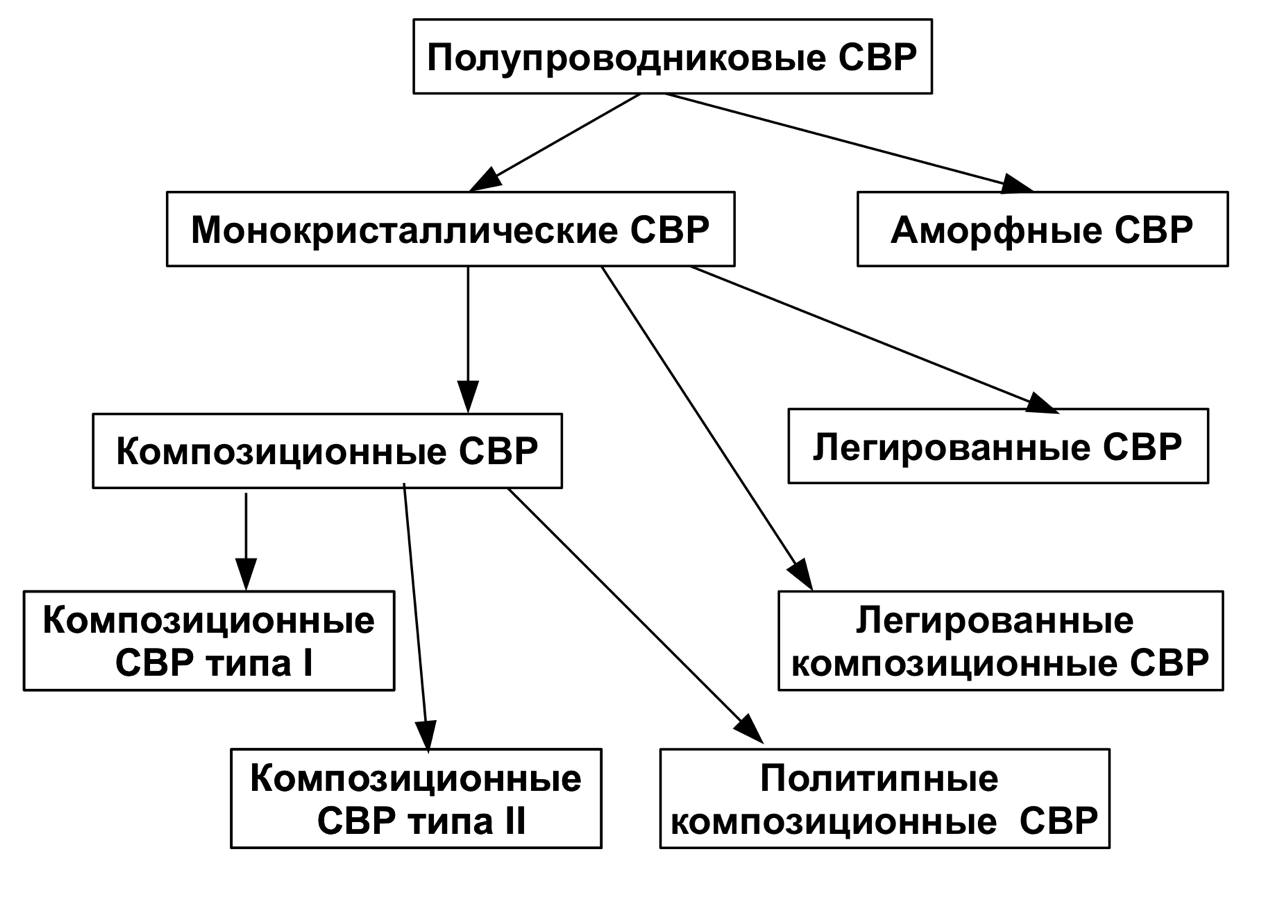
\includegraphics[width=0.5\textwidth]{images/ph30.4.jpg}
 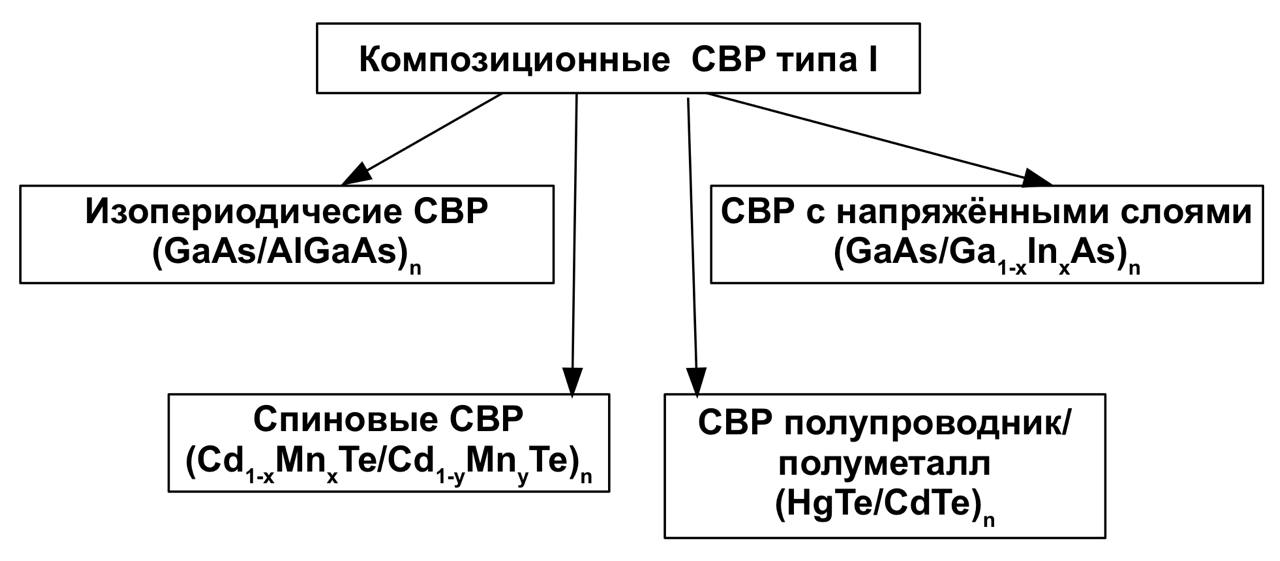
\includegraphics[width=0.5\textwidth]{images/ph30.5.jpg}
\end{figure}


\textbf{Энергетический спектр электронов в СВР}

Пример одномерной СВР с квадратичным изотропным законом дисперсии
исходных материалов. В направлении оси СВР за счёт перидического изменения потенциала зона Бриллюэна сжимается до интервала $2\pi / d$. На границах зоны Бриллюэна грууповая скорость обращается в 0, закон дисперсии разрывается, образуются \textbf{минизоны}, особенности плотности состояний (d - период СВР).
\begin{figure}[h!]
\centering
 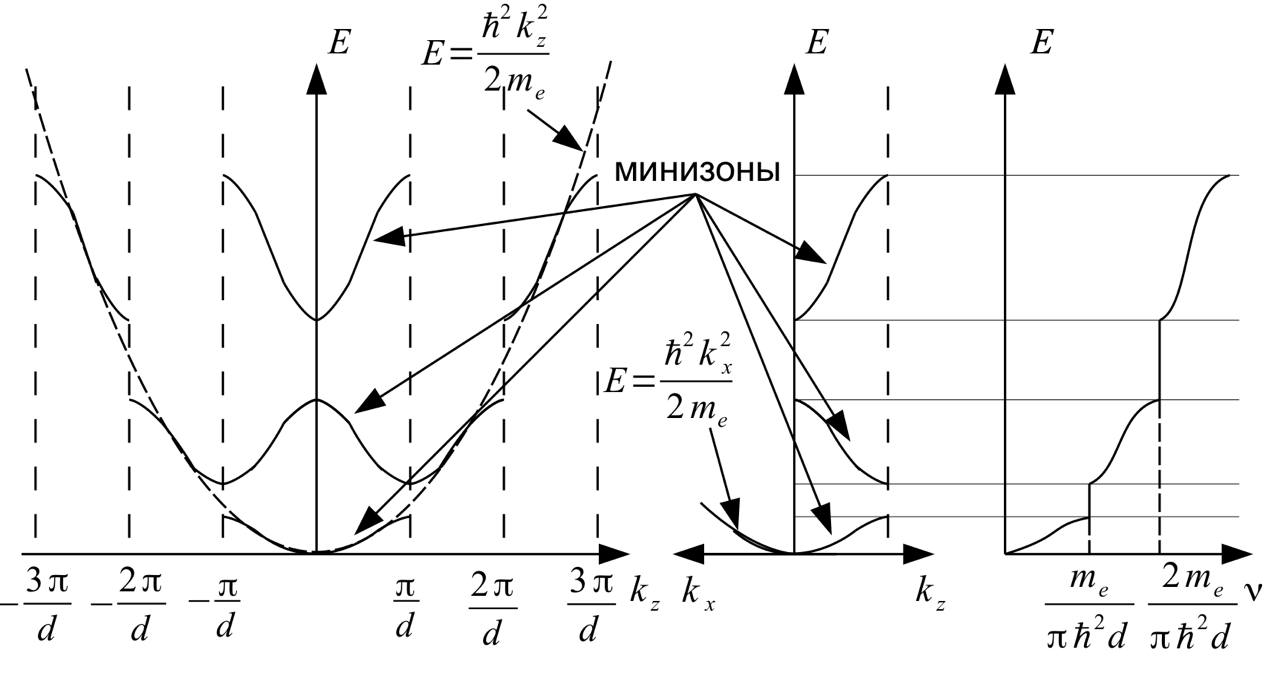
\includegraphics[width=\textwidth]{images/ph30.6.jpg}
\end{figure}

Из-за перекрытия волновых функций двумерные подзоны в квантовых
ямах превращаются в трёхмерные минизоны СВР. Волновые функции и
уровни энергии состояний в минизонах при слабом перекрытиии волновых
функций могут быть рассчитаны в рамках метода сильной связи:
\begin{figure}[h!]
\centering
 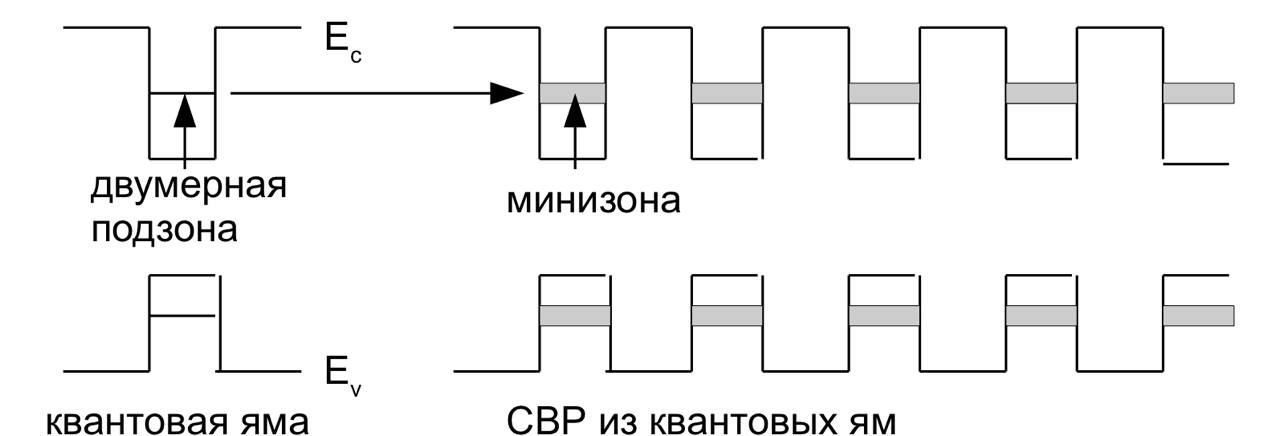
\includegraphics[width=\textwidth]{images/ph30.7.jpg}
\end{figure}


Волновая функция двумерной подзоны в одиночной квантовой ямы
$$
\psi_0(x, y, z)=\phi(z) \exp \left(i\left(k_x x+k_y y\right)\right)
$$
Волновая функция минизоны СВР в методе сильной связи
$$
\psi(x, y, z)=\sum_n \phi(z-n d) \exp \left(i n k_z d\right) \exp \left(i\left(k_x x+k_y y\right)\right)
$$
Закон дисперсии в рамках метода сильной связи
$$
E=\frac{\hbar^2\left(k_x^2+k_y^2\right)}{2 m_e}+E_0-2 t_E \cos \left(k_z d\right)
$$


\textbf{Электропроводность вдоль оси СВР. Осцилляции Блоха квазиклассический подход:}

Во внешнем электрическом поле напряжённости $G$ электрон за время $t$ в СВР приобретает дополнительный квазиимпульс:$\Delta p_z=e G t $
Средняя скорость электрона: $v_z=\frac{\partial E}{\partial p_z}$
Плотность тока: $j_z=\frac{2 e}{(2 \pi \hbar)^3} \int v_z d^3 p=j_z(e G t)$

Энергия, а значит и скорость и плотность тока периодическая орункция $p_z$. Период $T_{B I}$ и частота $f_{B l}$ осцилляций Блоха равны:
$$
e G T_{B l}=\frac{2 \pi \hbar}{d} \quad T_{B l}=\frac{2 \pi \hbar}{e G d} \quad f_{B l}=\frac{e G d}{2 \pi \hbar}
$$
Условия наблюдения:
$$
\begin{gathered}
T_{B l}<\tau \quad e G d<\Delta E \\
\Delta E-\text { ширина минизоны }
\end{gathered}
$$


Во внешнем электрическом поле напряжённости G периодичность
нарушается. В результате волновые функции состояний минизон
локализуются. Минизона распадается на систему дискретных уровней
энергии – лестницу Ванье-Штарка.
\begin{figure}[h!]
\centering
 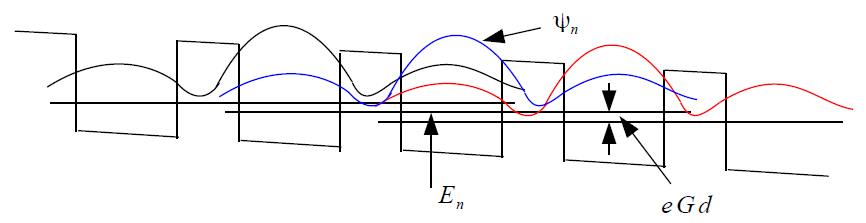
\includegraphics[width=\textwidth]{images/ph30.8.png}
\end{figure}

Уравнение Шредингера для СВР во внешнем электрическом поле
$$
\begin{gathered}
-\frac{\hbar^2}{2 m_1}\left(\frac{\partial^2 \psi}{\partial x^2}+\frac{\partial^2 \psi}{\partial y^2}+\frac{\partial^2 \psi}{\partial z^2}\right)-e G z \psi=E \psi \quad \text { яма } \\
-\frac{\hbar^2}{2 m_2}\left(\frac{\partial^2 \psi}{\partial x^2}+\frac{\partial^2 \psi}{\partial y^2}+\frac{\partial^2 \psi}{\partial z^2}\right)+\left(\Delta E_c-e G z\right) \psi=E \psi \quad \text { барьер }
\end{gathered}
$$


Волновая функция
$$
\psi_n=\exp \left(i\left(k_x x+k_y y\right)\right) \sum_m c_m \phi(z-m d)
$$
$\phi(z)$ - функция, описывающая зависимость волновой функции от z в ненулевом электричесқом поле
$$
c_m=J_{n-m}\left(\frac{\Delta E}{e G d}\right) \approx \frac{1}{|n-m| !}\left(\frac{\Delta E}{2 e G d}\right)^{|n-m|}
$$
Уровни энергии
$$
E_n=E_0+n e G d, \mathrm{n}=0, \pm 1, \pm 2, \ldots
$$
Квантовое описание осцилляций. Построим нестационарное состояние из волновых функций двух соседних состояний в электрическом поле
$$
\psi=a_1 \psi_1 \exp \left(\frac{i E_0 t}{\hbar}\right)+a_2 \psi_2 \exp \left(\frac{i\left(E_0+e G d\right) t}{\hbar}\right)
$$
Плотность вероятности
$$
|\psi|^2=\left|a_1\right|^2 \psi_1^2+\left|a_2\right|^2 \psi_2^2+2 a_1 a_2 \psi_1 \psi_2 \cos \left(\frac{e G d t}{\hbar}\right)
$$
Среднее значение координаты $z$ также осциллирует с частотой Блоха
$$
\bar{z}=\int z|\psi|^2 d z \approx \bar{z}_1+\bar{z}_2+2 a_1 a_2 z_0 c \cos \left(\frac{e G d t}{\hbar}\right) z_0 c=\int z \psi_1 \psi_2 d z
$$
Стационарная электропроводность в режиме осцилляций Блоха:

Без учёта релаксации импульса постоянный ток в режиме осцилляций не течёт. Учтём релаксацию импульса в простейщем приближении, считая, что скорость релаксирует по тому же закону, что и импульс. Для стационарной скорости:
$$
v_z(\infty)=\int_0^{\infty} \exp (-t / \tau) d v_z(t)
$$
Вычислим для закона дисперсии в приближении сильной связи
$$
\begin{gathered}
E=E_0-2 t_E \cos \left(\frac{e G t}{\hbar} d\right) \\
d v_z(t)=\frac{d^2 E}{d p_z^2} d p_z(t)=\frac{2 t_E d^2}{\hbar^2} e G \cos \left(\frac{e G t}{\hbar} d\right) d t
\end{gathered}
$$
После интегрирования получаем:
$$
\begin{aligned}
v_z(\infty)=\int_0^{\infty} \exp (-t / \tau) d v_z(t) & =\frac{2 t_E d}{\hbar} \int_0^{\infty} \exp \left(-\frac{x}{\omega_{B l} \tau}\right) \cos x d x=\frac{2 t_E d}{\hbar} \frac{\omega_{B l} \tau}{1+\left(\omega_{B l} \tau\right)^2} \\
\omega_{B l} & =2 \pi f_{B l}=\frac{e G d}{\hbar}
\end{aligned}
$$

\textbf{Отрицательная дифференциальная проводимость в режиме
осцилляций Блоха:}
\begin{figure}[h!]
\centering
 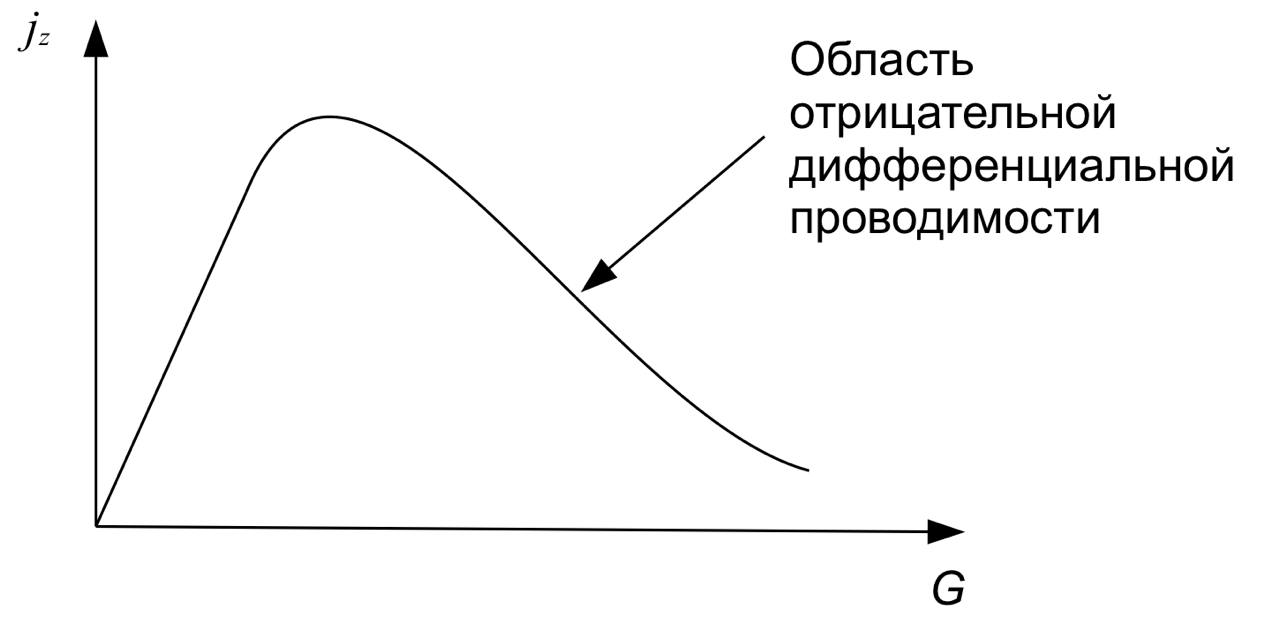
\includegraphics[width=0.5\textwidth]{images/ph30.9.jpg}
\end{figure}

$j_z=e n v_z(\infty), n$ - концентрация электронов в минизоне
В области отрицательной диффреренциальной проводимости равномерное распределение электрического поля в СВР неустойчиво. Поле концентрируется в некоторых областях доменах. Домены могут двигаться при протекании тока

\textbf{Резонансное туннелирование в СВР}

\begin{figure}[h!]
\centering
 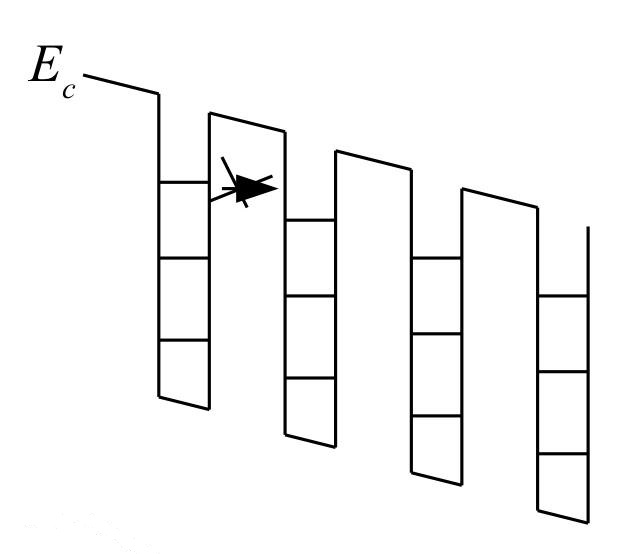
\includegraphics[width=0.4\textwidth]{images/ph30.10.1.jpg}
 \caption*{При условии $eGd > \Delta E$ минизона
разрушается. При этом электрический
ток и элеткропроводность минимальны}
\end{figure}

\begin{figure}[h!]
\centering
 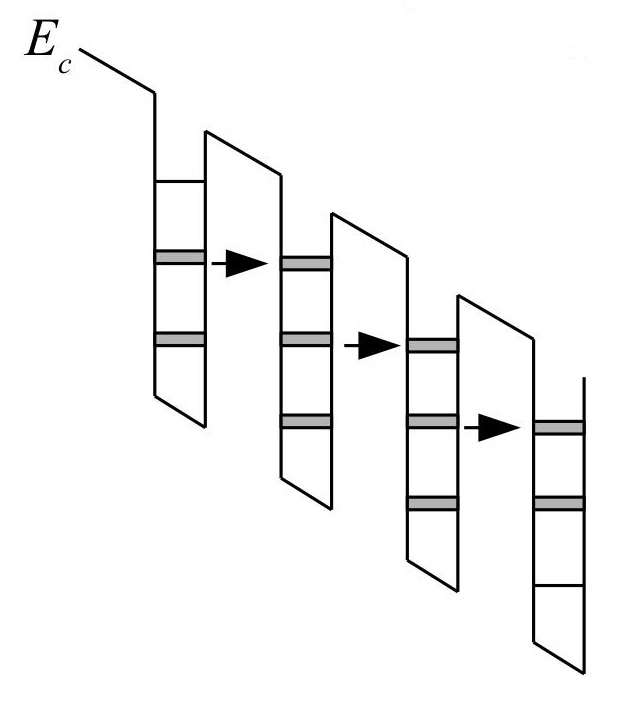
\includegraphics[width=0.4\textwidth]{images/ph30.10.2.jpg}
 \caption*{При наличии нескольких минизон
дальнейшее увеличение поля может
привести к выполнению условия
$eGd =E_2-E_1 $ возникает резонансное
туннелирование, уровни в
потенциальных ямах уширяются,
электрический ток и
электропроводность увеличиваются}
\end{figure}


\textbf{Отрицательная дифференциальная проводимость перпендикулярно оси СВР}
\begin{figure}[h!]
\centering
 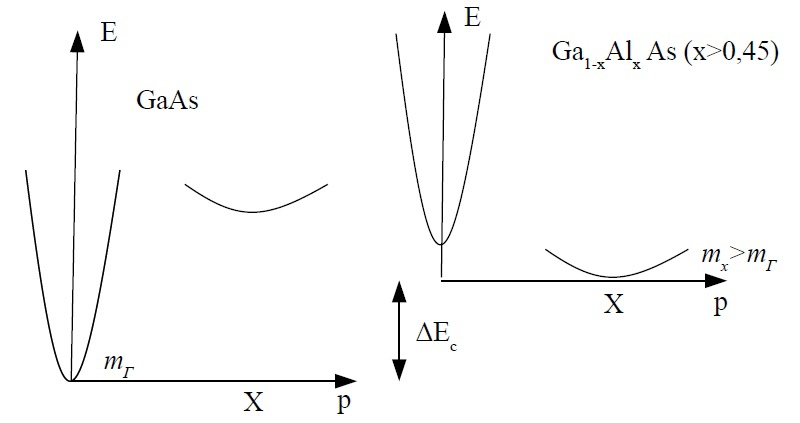
\includegraphics[width=0.8\textwidth]{images/ph30.11.jpg}
\end{figure}
$Ga_{1-x}Al_xAs$
При увеличении содержания Al до $\mathrm{x}=0,45$ минимум зоны проводимости в точках X становится основным. Эффективная масса электронов в X-минимуме намного больше чем в Г-минимуме. Таким образом при x>0,45 масса электронов в барьерных слоях намного больше, чем в слоях потенциальных ям.



\begin{figure}[h!]
\centering
 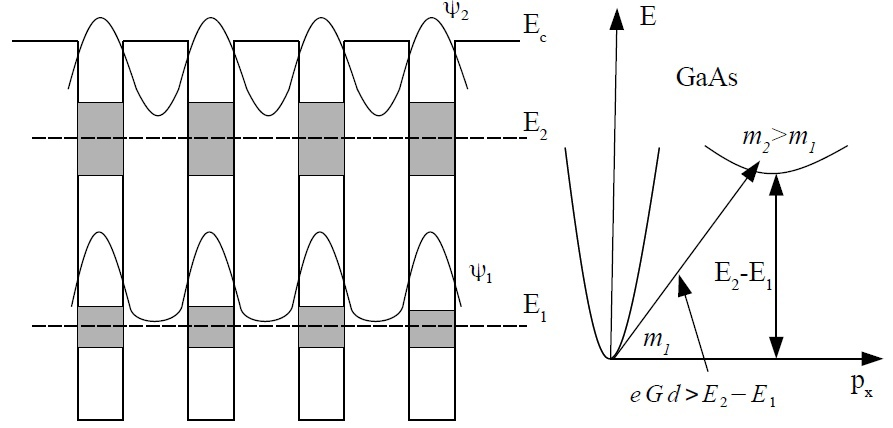
\includegraphics[width=0.8\textwidth]{images/ph30.12.jpg}
\end{figure}
Волновые функции верхних минизон СВР глубже проникают в барьерные слои.
Поэтому эффективная масса электронов в верхних минизонах значительно
больше чем в нижних. В достаточно сильном электрическом поле электроны
приобретают достаточно энергии для перехода в верхнюю минизону. При этом
подвижность электронов и электропроводность резко падают. Это отрицательная
дифференциальная проводимость. 


\section{Графен. Структура графена. Точки Дирака. Закон дисперсии для электронов и дырок.  Целочисленный квантовый эффект Холла в графене.}

K веществам, имеющим двумерную или хвазидвумерную электронную структуру относится графит и его интеркалированные соединения. 

\textbf{Структура графена:}

Атомы углерода в графите располагаются в параллельных слоях, расстояние между которыми при комнатной температуре составляет $d_0=0,36$ нм. В каждом плоском слое атомы углерода образуют сетку правильньх шестиугальников, с расстоянием между атомами $\mathrm{C}-\mathrm{C}$ равным $\mathrm{b}_0=0.14$ нм. В каждом последующем слое атомы смещены так, что часть из них расположена под центрами шестиугольников, а частьпод атомами вьшележащего слоя. Такая структура соответствует гексагональной решетке с четырьмя атомами углерода в элементарной ячейке.
\begin{figure}[h!]
\centering
 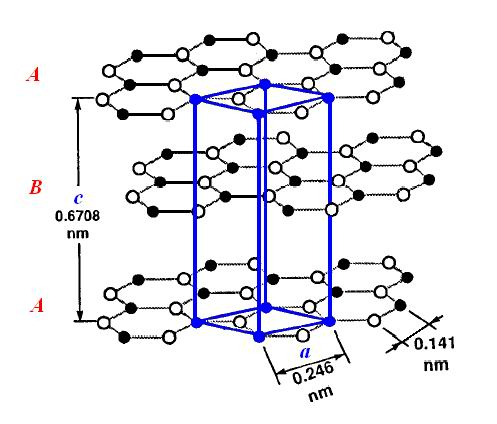
\includegraphics[width=0.4\textwidth]{images/ph31.1.jpg}
\end{figure}

Поскольку взаимодействие атомов утлерода в одном слое значительно сильнее их взаимодействия в соседних слоях, то хорошим приблихением зонной структуры графита является двумерная модель (=графен). 

\textbf{Энергетический спектр:}

В гексагональной модификации в элементарной ячейке 4 неэквивалентных
атома, по два из каждого графенового слоя. В результате перекрытия
волновых функций слоёв законы дисперсии для электронов и дырок
вблизи т. K должны расщепляться. Электроны из отщеплённой вверх ветви
валентной зоны переходят в отщеплённую вниз ветвь зоны проводимости. Точка К --- \textbf{точка Дирака.}
В результате графит – полуметалл.
\begin{figure}[h!]
\centering
 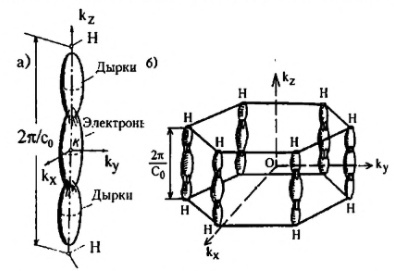
\includegraphics[width=0.6\textwidth]{images/ph31.2.jpg}
 \caption*{Поверхность Ферми графита (а) и ее расположение в зоне Бриллюэна (6)}
\end{figure}


На рисунке приведена первая зона Бриллюэна графита и поверхность Ферми, состоящая из электронных (в точке К) и дырочных (достигающих точки Н) элипсоидов (по два эллипсоида на зону).

\begin{figure}[h!]
\centering
 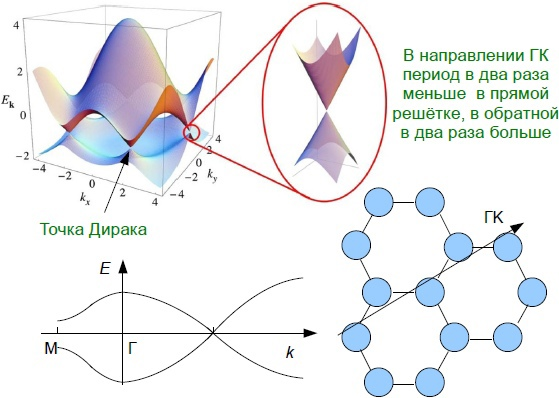
\includegraphics[width=\textwidth]{images/ph31.3.jpg}
 \caption*{Графен. Закон дисперсии. Графическое представление}
\end{figure}


\textbf{Закон дисперсии:}
Площадь занимая состояниями с энергией $E^{\prime}<E$ в р-пространстве
$$
S\left(E^{\prime}<E\right)=\pi\left(\frac{E}{v_0}\right)^2
$$
Концентрация состояний с энергией $E^{\prime}<E$
$$
N\left(E^{\prime}<E\right)=\frac{4 S\left(E^{\prime}<E\right)}{(2 \pi \hbar)^2}=\frac{1}{\pi \hbar^2}\left(\frac{E}{v_0}\right)^2
$$
Плотность состояний:
$$
v(E)=\frac{\partial N\left(E^{\prime}<E\right)}{\partial E}=\frac{4 S\left(E^{\prime}<E\right)}{(2 \pi \hbar)^2}=\frac{2 E}{\pi \hbar^2 v_0^2}
$$
Концентрация электронов (дырок) в случае вырожденной статистики при заданном положении уровня Ферми
$$
n_{2 \mathrm{D}}=\frac{1}{\pi \hbar^2}\left(\frac{F^2}{v_0^2}\right)
$$
Концентрация электронов в нелегированном графене
$$
n_{2 \mathrm{D}}=p_{2 \mathrm{D}}=\int_0^{\infty} v(E) f_0(E) d E
$$
Вблизи точки Дирака законы дисперсии (плотность состояний) для электронов и дырок симметричны, поэтому для электронейтральности должно быть $F=0$
$$
\begin{gathered}
n_{2 D}=p_{2 D}=\frac{2}{\pi \hbar^2 v_0^2} \int_0^{\infty} \frac{E d E}{\exp \left(\frac{E}{k_B T}\right)+1}=\frac{\left(k_b T\right)^2}{\pi \hbar^2 v_0^2} \int_0^{\infty} \frac{x d x}{\exp (x)+1}=\frac{C\left(k_B T\right)^2}{\pi \hbar^2 v_0^2} \\
C=2 \int_0^{\infty} \frac{x d x}{\exp (x)+1}=\frac{\pi^2}{6}-\text { число }
\end{gathered}
$$

\textbf{Целочисленный квантовый эффект Холла в графене:}
Рассмотрим процесс квантования энергии электронов в графене в магнитном поле.
Квазиклассическое условие квантования площадей:
$$
S_n=\pi\left(\frac{E_n}{v_0}\right)^2=2 \pi \hbar e B(n+\gamma)
$$
Уровни Ландау в квазиклассическом приближении:
$$
E_n= \pm v_0 \sqrt{2 \hbar e B(n+\gamma)}
$$
Точное решение уравнения Дирака в магнитном поле:
$$
E_n= \pm v_0 \sqrt{2 \hbar e B n}, n=0,1,2,3 \ldots
$$
Кратность вырождения уровня без учёта спинового расщепления:
$$
N_L=\frac{2}{2 \pi l_B^2}, n=0 \quad N_L=\frac{4}{2 \pi l_B^2}, n>0
$$
Период осцилляции сопротивления в зависимости от концентрации электронов в постоянном магнитном поле
$$
n_{2 D n}=\frac{1}{\pi \hbar^2} \frac{F^2}{v_0^2}=\frac{2 e B n}{\pi \hbar} \quad n_{2 D n+1}=\frac{1}{\pi \hbar^2} \frac{F^2}{v_0^2}=\frac{2 e B(n+1)}{\pi \hbar}
$$
Отсюда находим:
$$
\left(n_{2 \mathrm{D}+1}-n_{2 \mathrm{Dn}}\right) \frac{\pi \hbar}{2 e B}=1 \quad  T_n=n_{2 \mathrm{Dn}+1}-n_{2 \mathrm{Dn}}=\frac{\pi \hbar}{2 e B}=\frac{2 e B}{\pi \hbar}
$$

Тогда квантование холловской проводимости:
$$
\sigma_H=\frac{4 e^2}{2 \pi \hbar}\left(v+\frac{1}{2}\right), v=1,2, \ldots
$$

\begin{figure}[h!]
\centering
 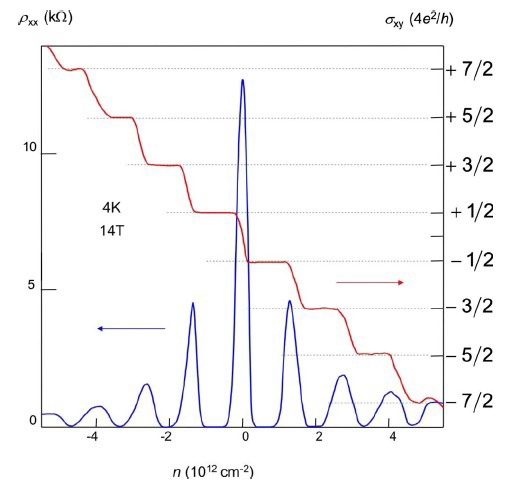
\includegraphics[width=0.7\textwidth]{images/ph31.4.jpg}
\end{figure}